
\section{Examples}

\textbf{About:} This section will run the user through some examples of what this program is capable of along with some higher level discussion about what is going on in each step. Note that these examples are here to demonstrate bertini and bertini\_real using the instructions prior to this, so there will not be any step by step analysis here.
	
\subsection{Curves}


\subsubsection{Circle}

\paragraph{Input file}

	\File{Presents an input file from circle that instructs Bertini to use all default settings to compute the numerical irreducible decomposition of the sphere in two dimensions}{asdf}{../../test/curve/circle/input}

\paragraph{Decomposition}
	
	\begin{figure}[H]\centering
	     \frame{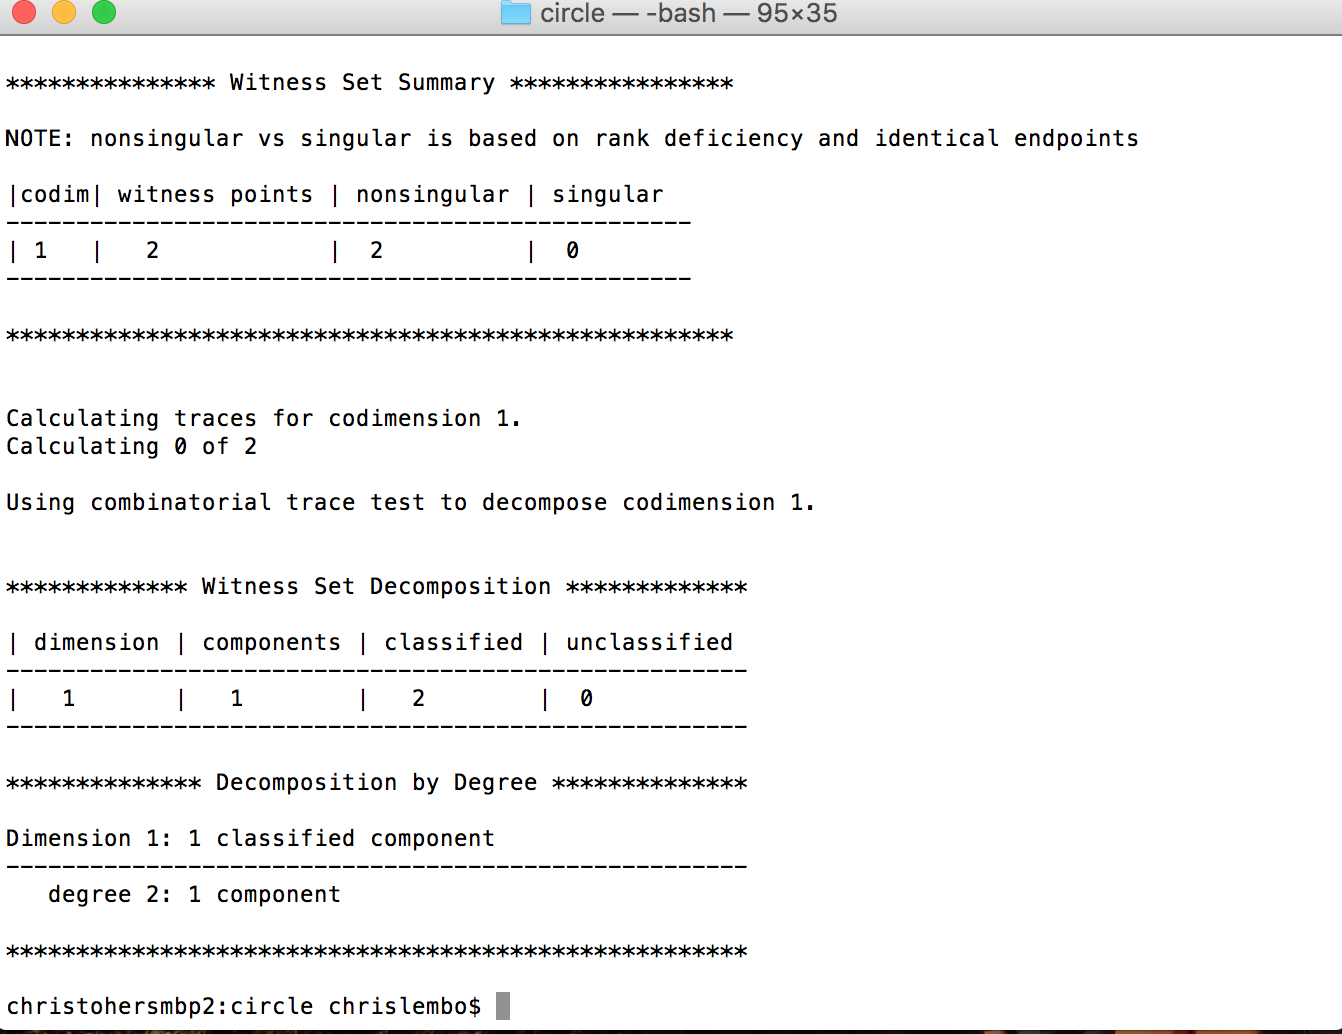
\includegraphics[width=10cm]{example1decomp1}}
	     \caption{Running Bertini using the Circle input file}
	\end{figure}

	\begin{figure}[H]\centering
	     \frame{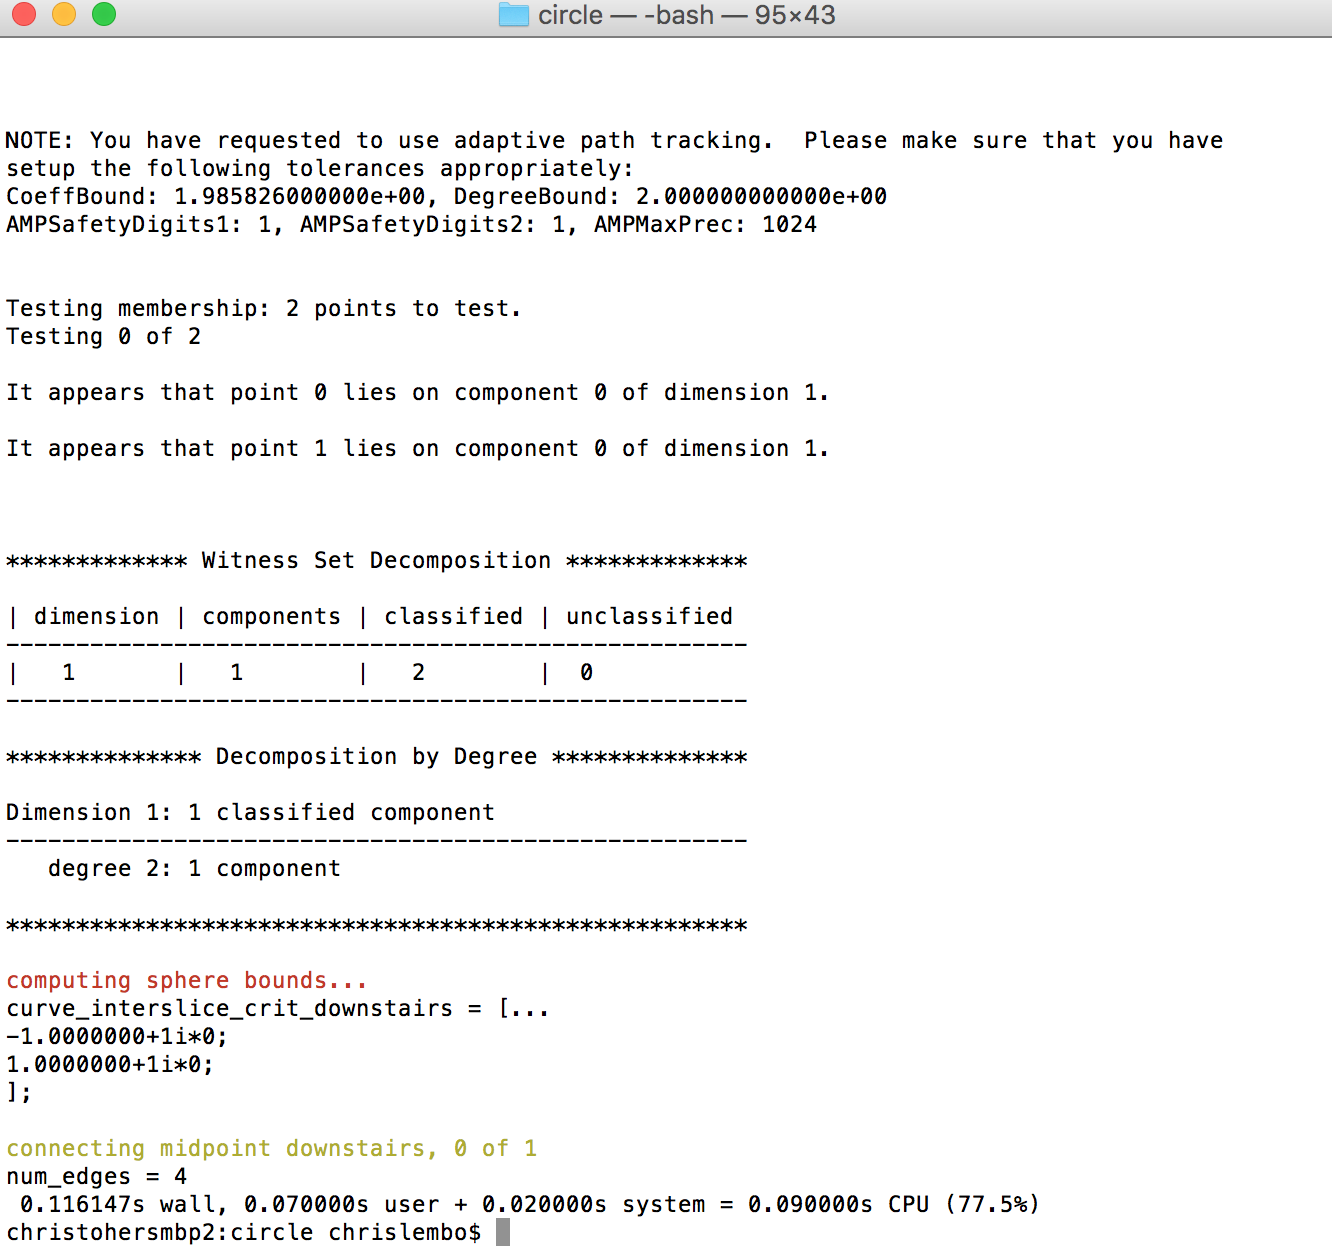
\includegraphics[width=10cm]{example1decomp2}}
	     \caption{Running Bertini\_real using the Circle input file}
	\end{figure}
		
\paragraph{Refinement}

	\begin{figure}[H]\centering
	     \frame{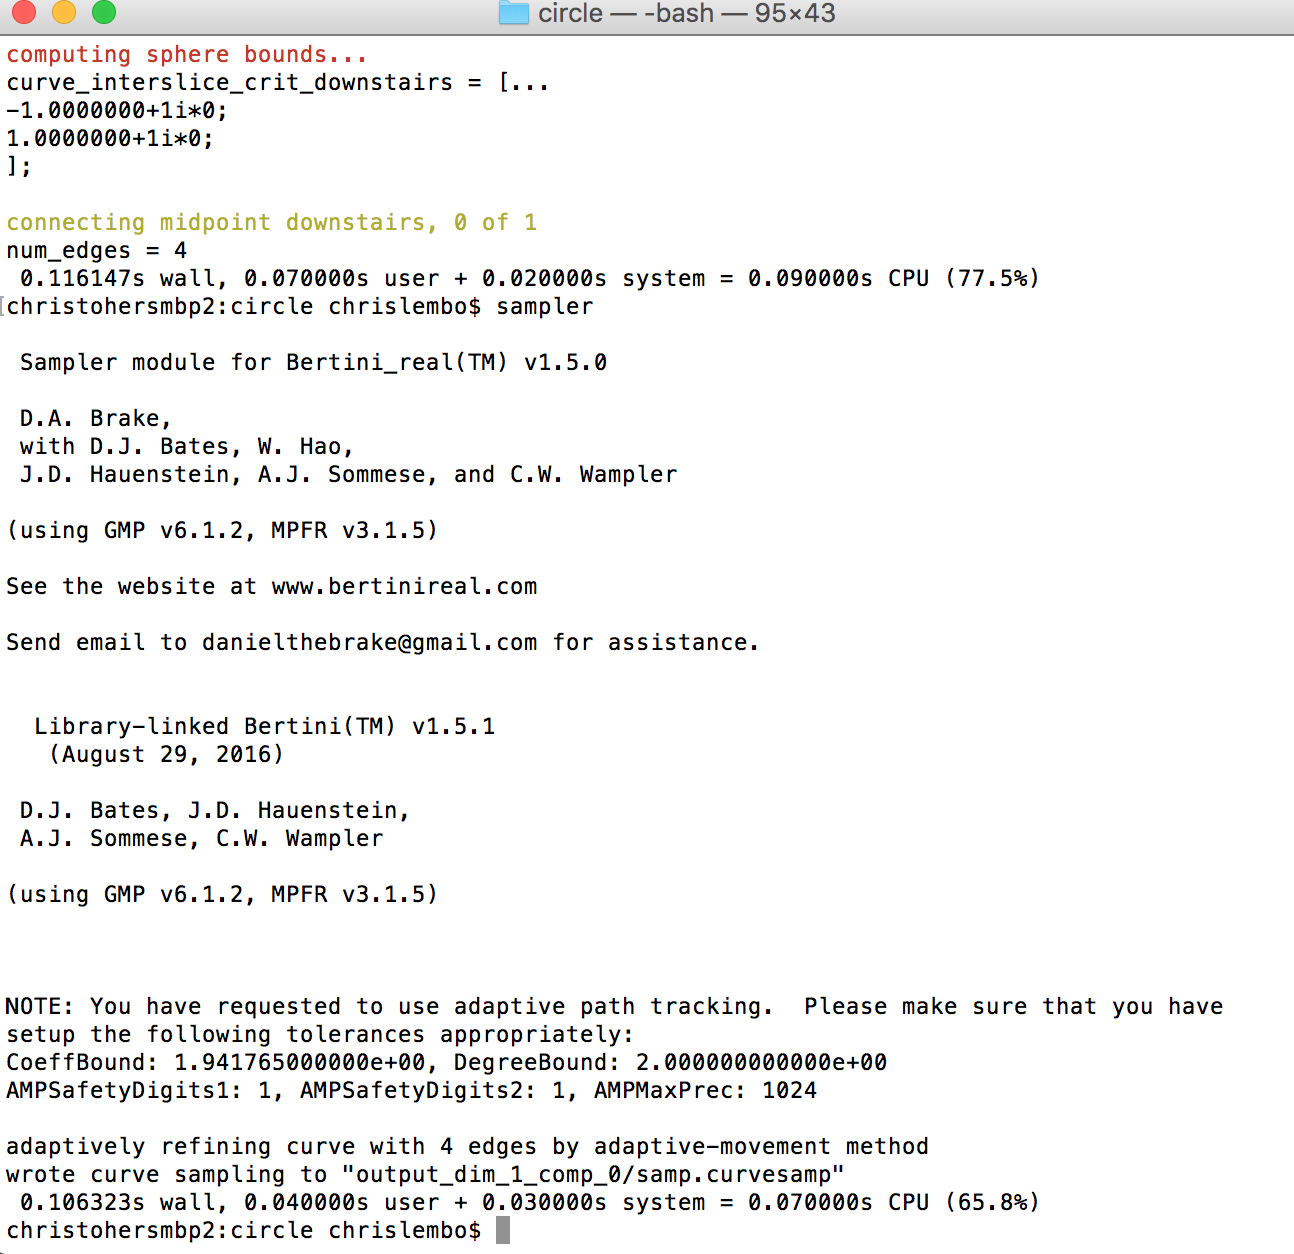
\includegraphics[width=10cm]{example1ref1}}
	     \caption{Refining the Circle input file by invoking sampler}
	\end{figure}

	\begin{figure}[H]\centering
	     \frame{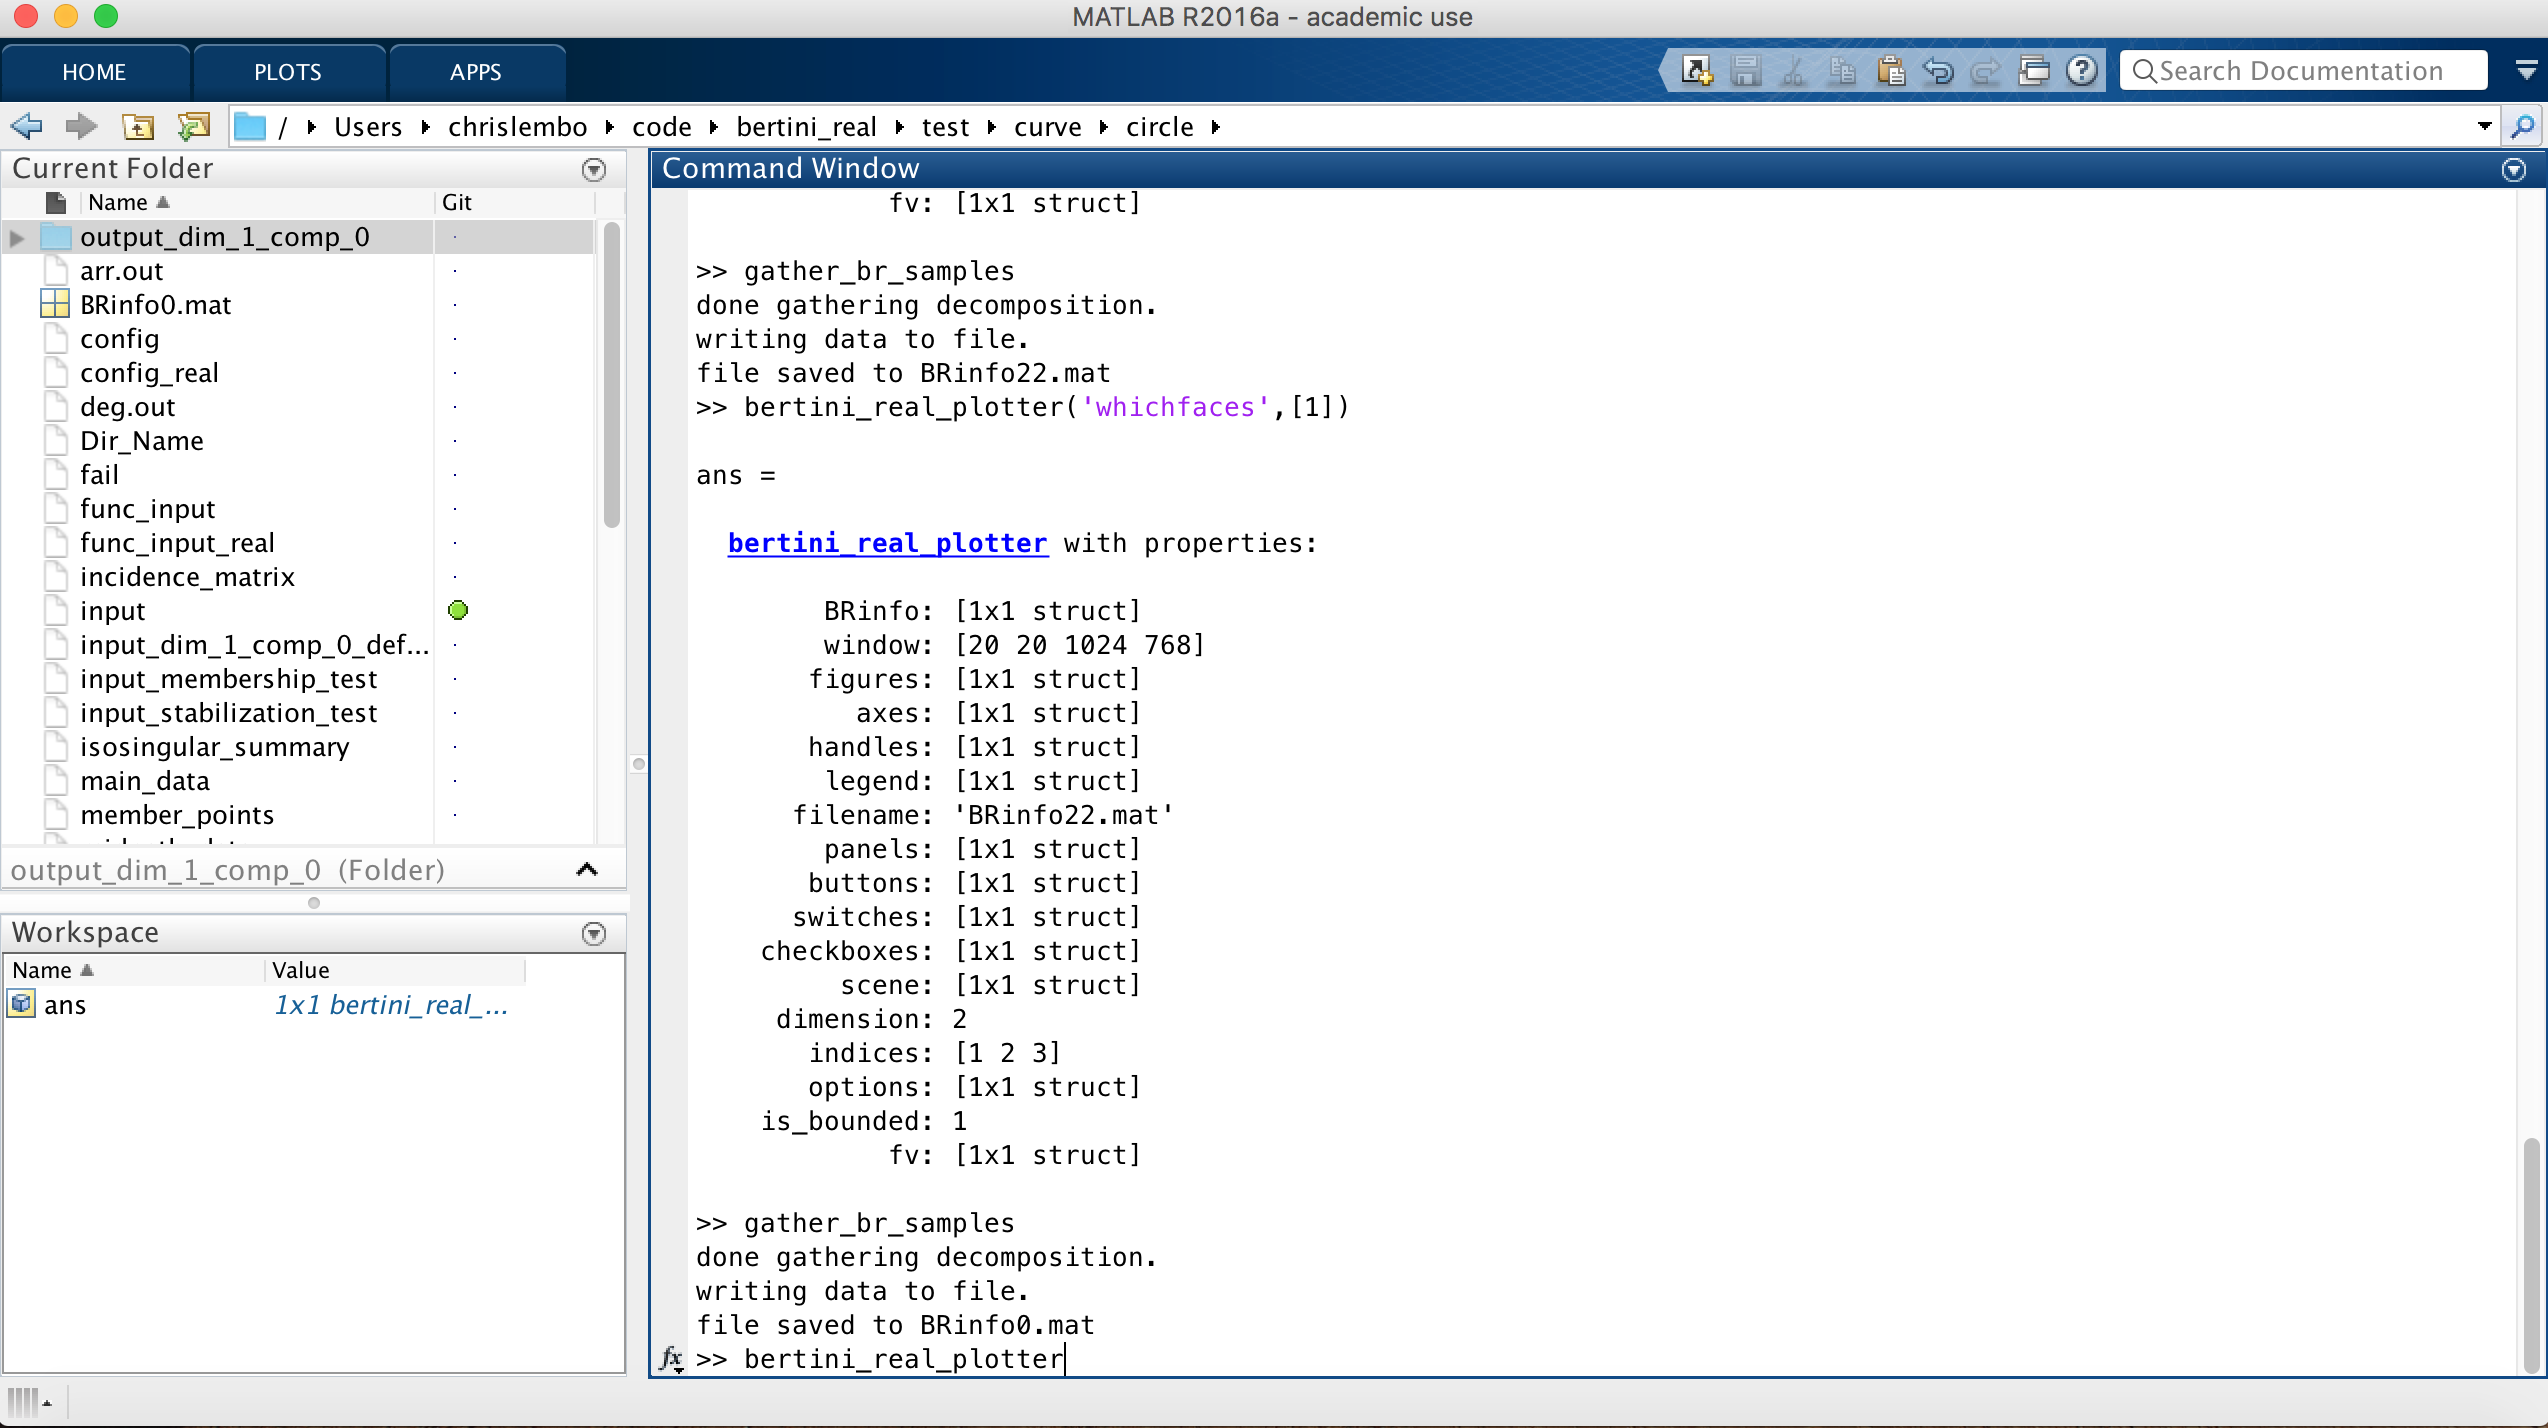
\includegraphics[width=10cm]{example1ref2}}
	     \caption{Gathering and Plotting using MATLAB}
	\end{figure}

	\begin{figure}[H]\centering
	     \frame{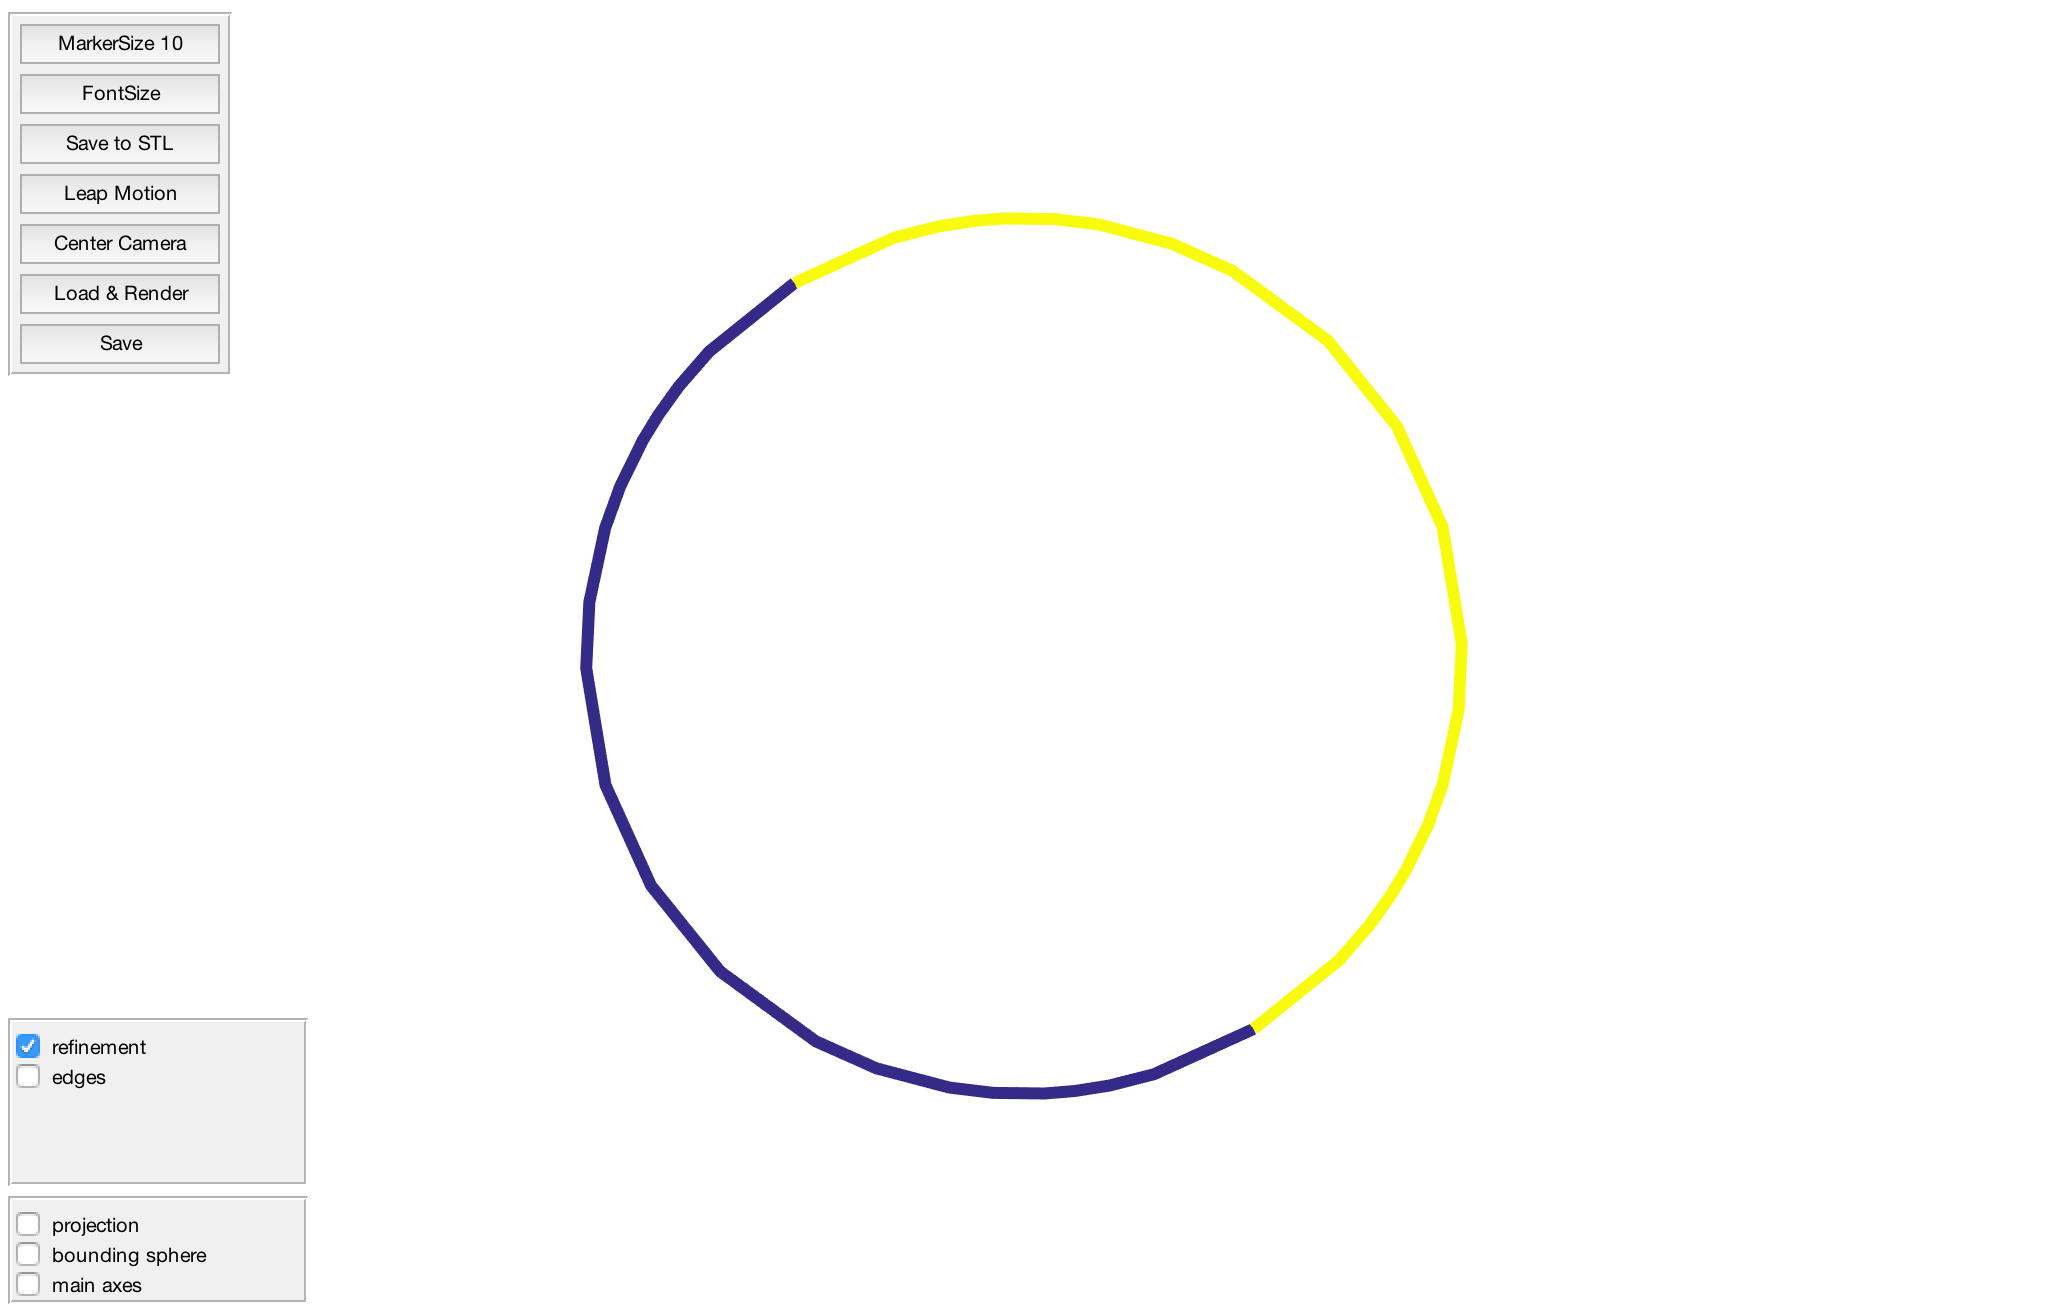
\includegraphics[width=10cm]{example1ref3.png}}
	     \caption{Final Circle plotted}
	\end{figure}

\paragraph{Notes}

%not sure what to put here

\subsubsection{Astroid}

\paragraph{Input file}

	\File{Presents an input file from astroid that instructs Bertini to use all default settings to compute the numerical irreducible decomposition of the sphere in one dimension}{asdf}{../../test/curve/astroid/input}

\paragraph{Decomposition}
	
	\begin{figure}[H]\centering
	    \frame{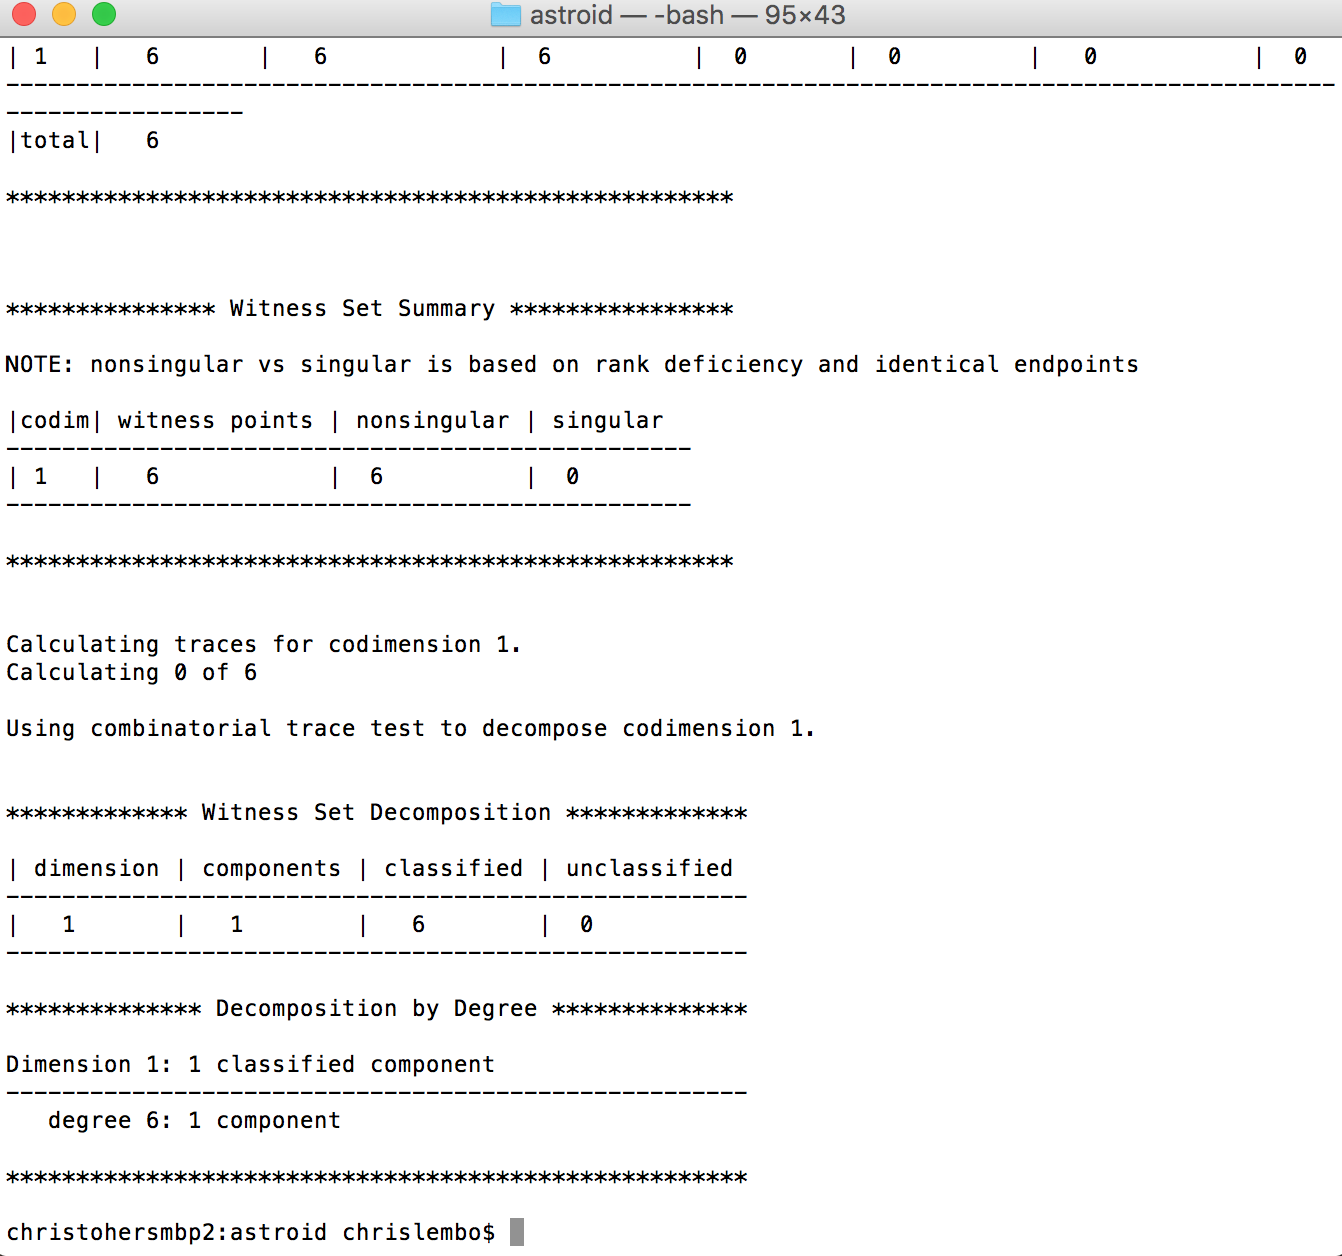
\includegraphics[width=10cm]{example2decomp1}}
	    \caption{Running Bertini using the astroid input file}
	\end{figure}

	\begin{figure}[H]\centering
	    \frame{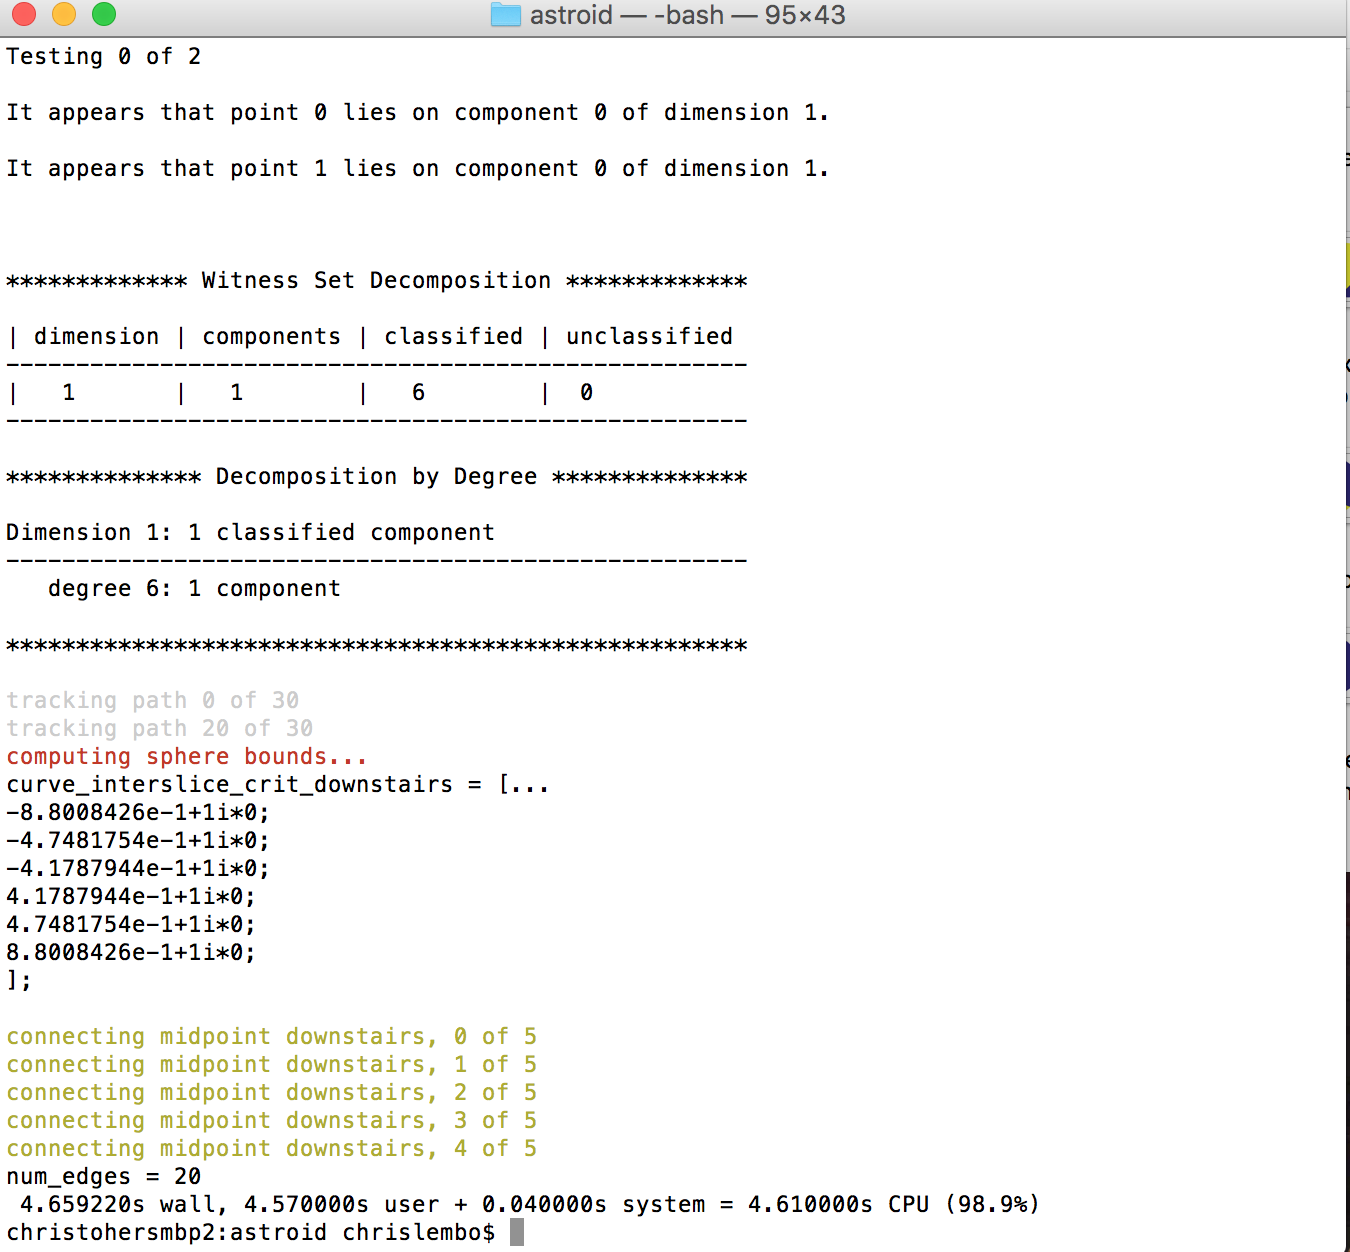
\includegraphics[width=10cm]{example2decomp2}}
	    \caption{Running Bertini\_real using the astroid input file}
	\end{figure}
		
\paragraph{Refinement}

	\begin{figure}[H]\centering
	    \frame{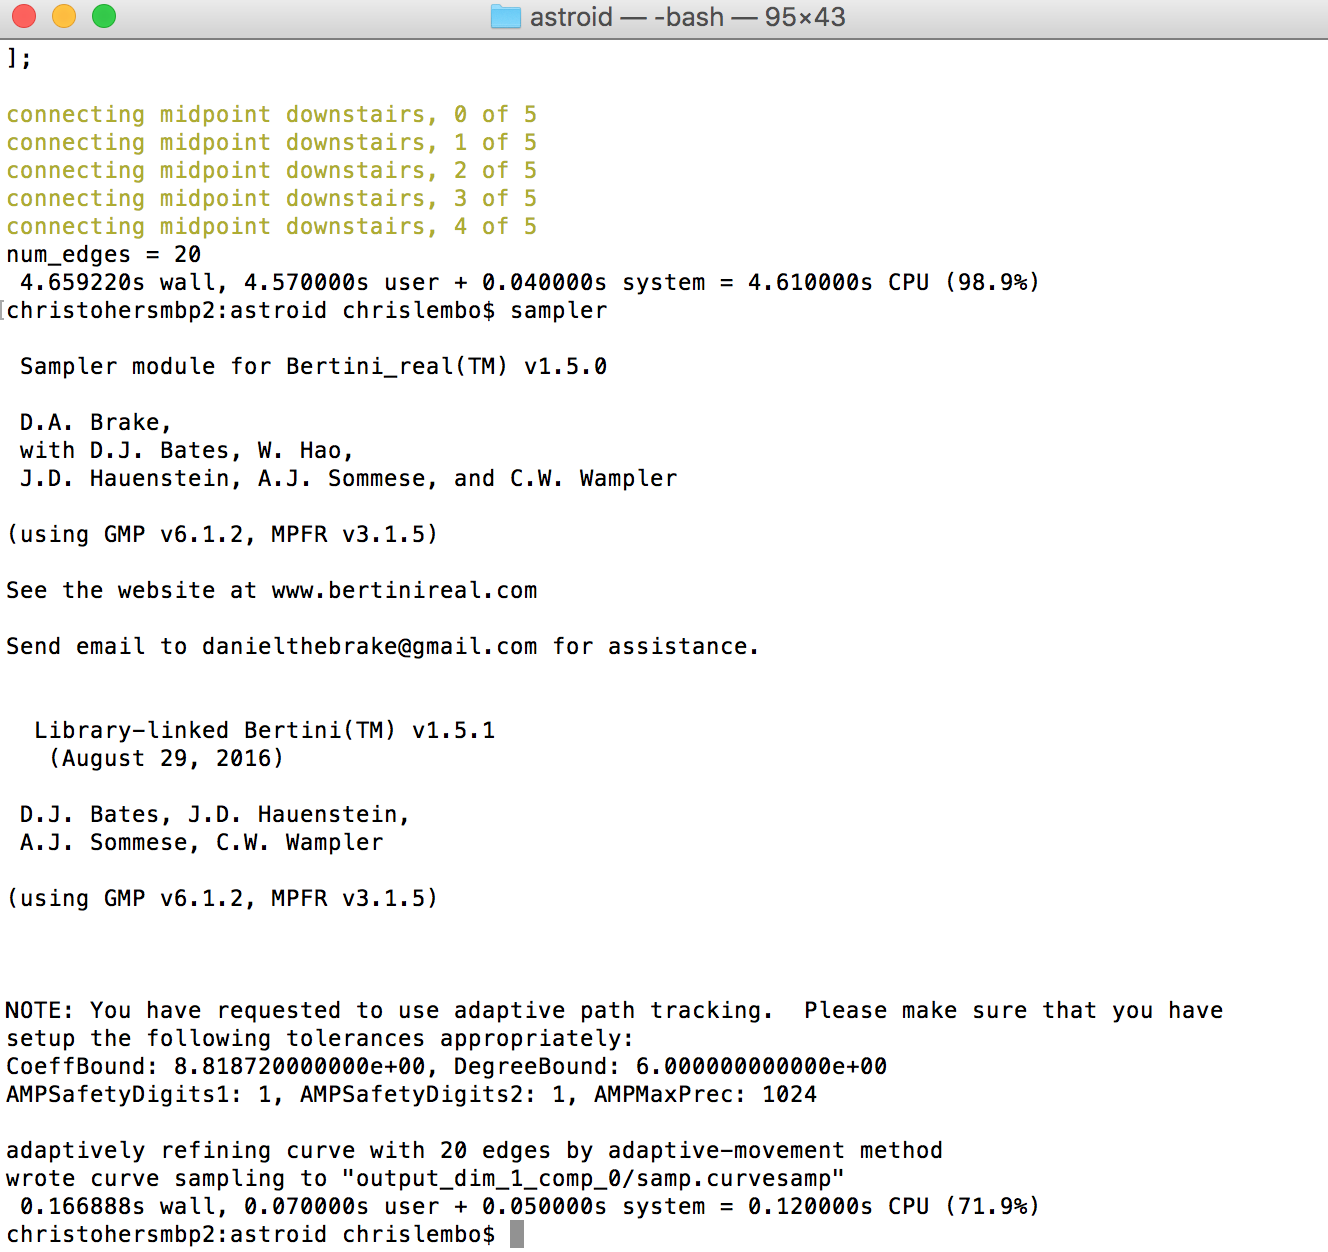
\includegraphics[width=10cm]{example2ref1}}
	    \caption{Refining the astroid input file by invoking sampler}
	\end{figure}

	\begin{figure}[H]\centering
	    \frame{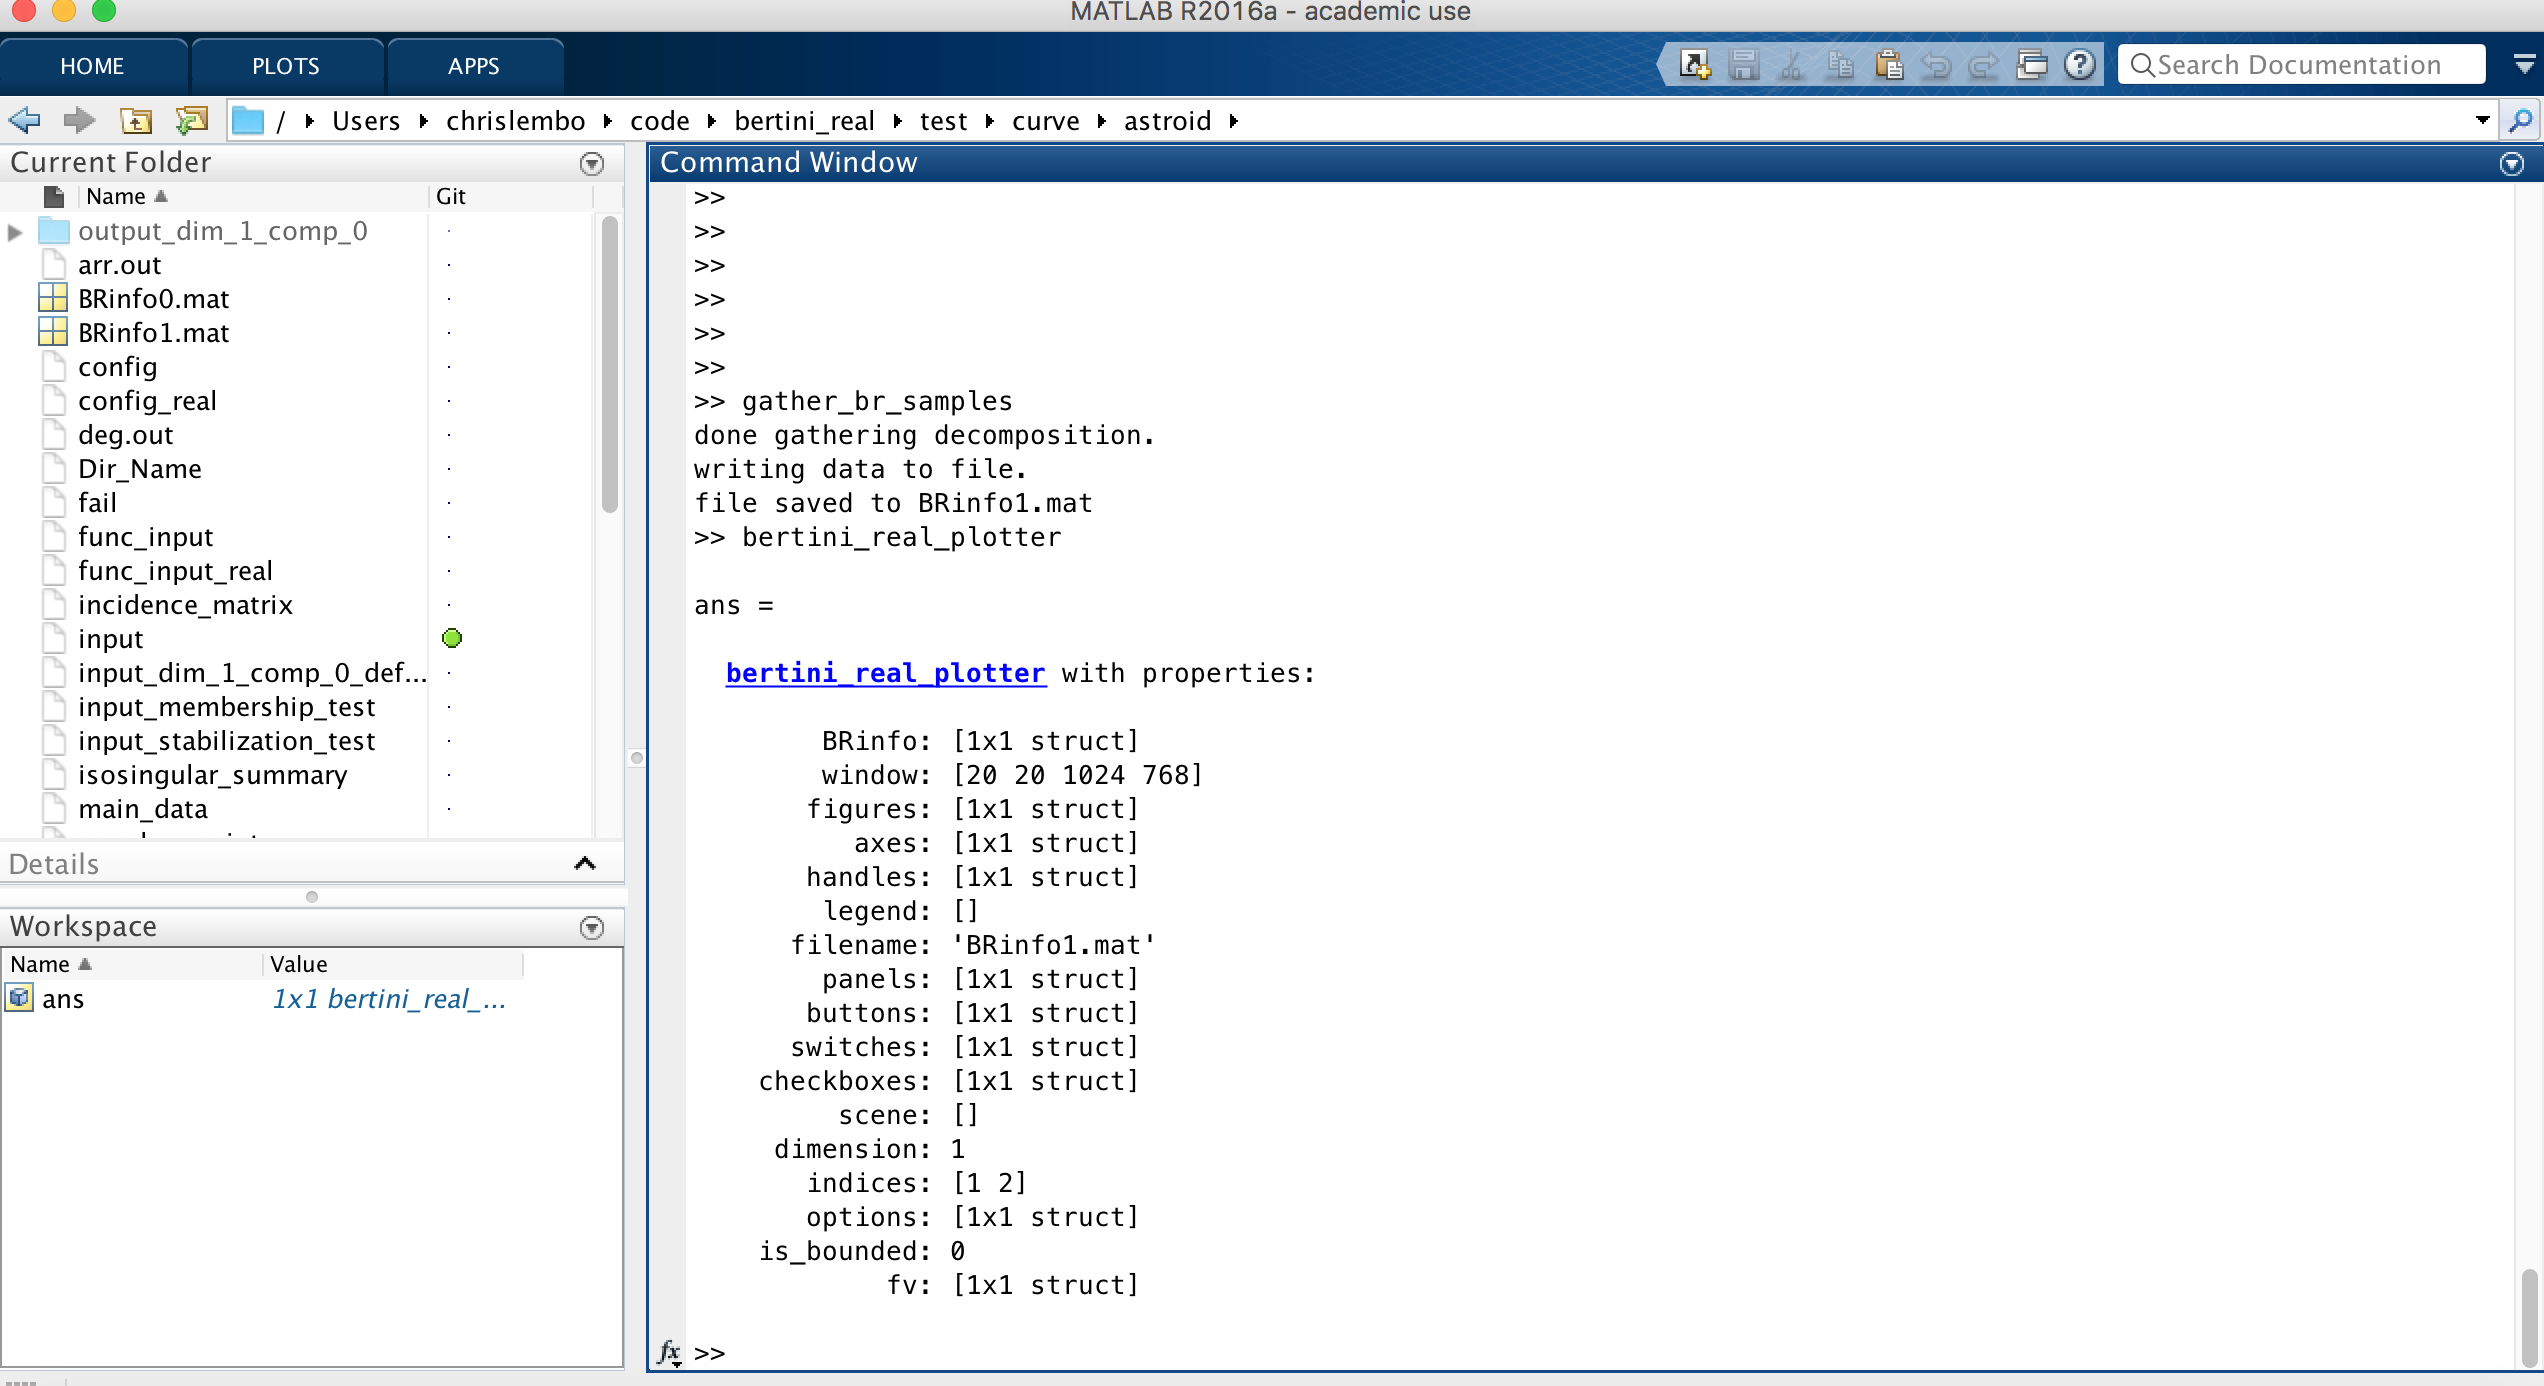
\includegraphics[width=10cm]{example2ref2}}
	    \caption{Gathering and Plotting using MATLAB}
	\end{figure}

	\begin{figure}[H]\centering
	    \frame{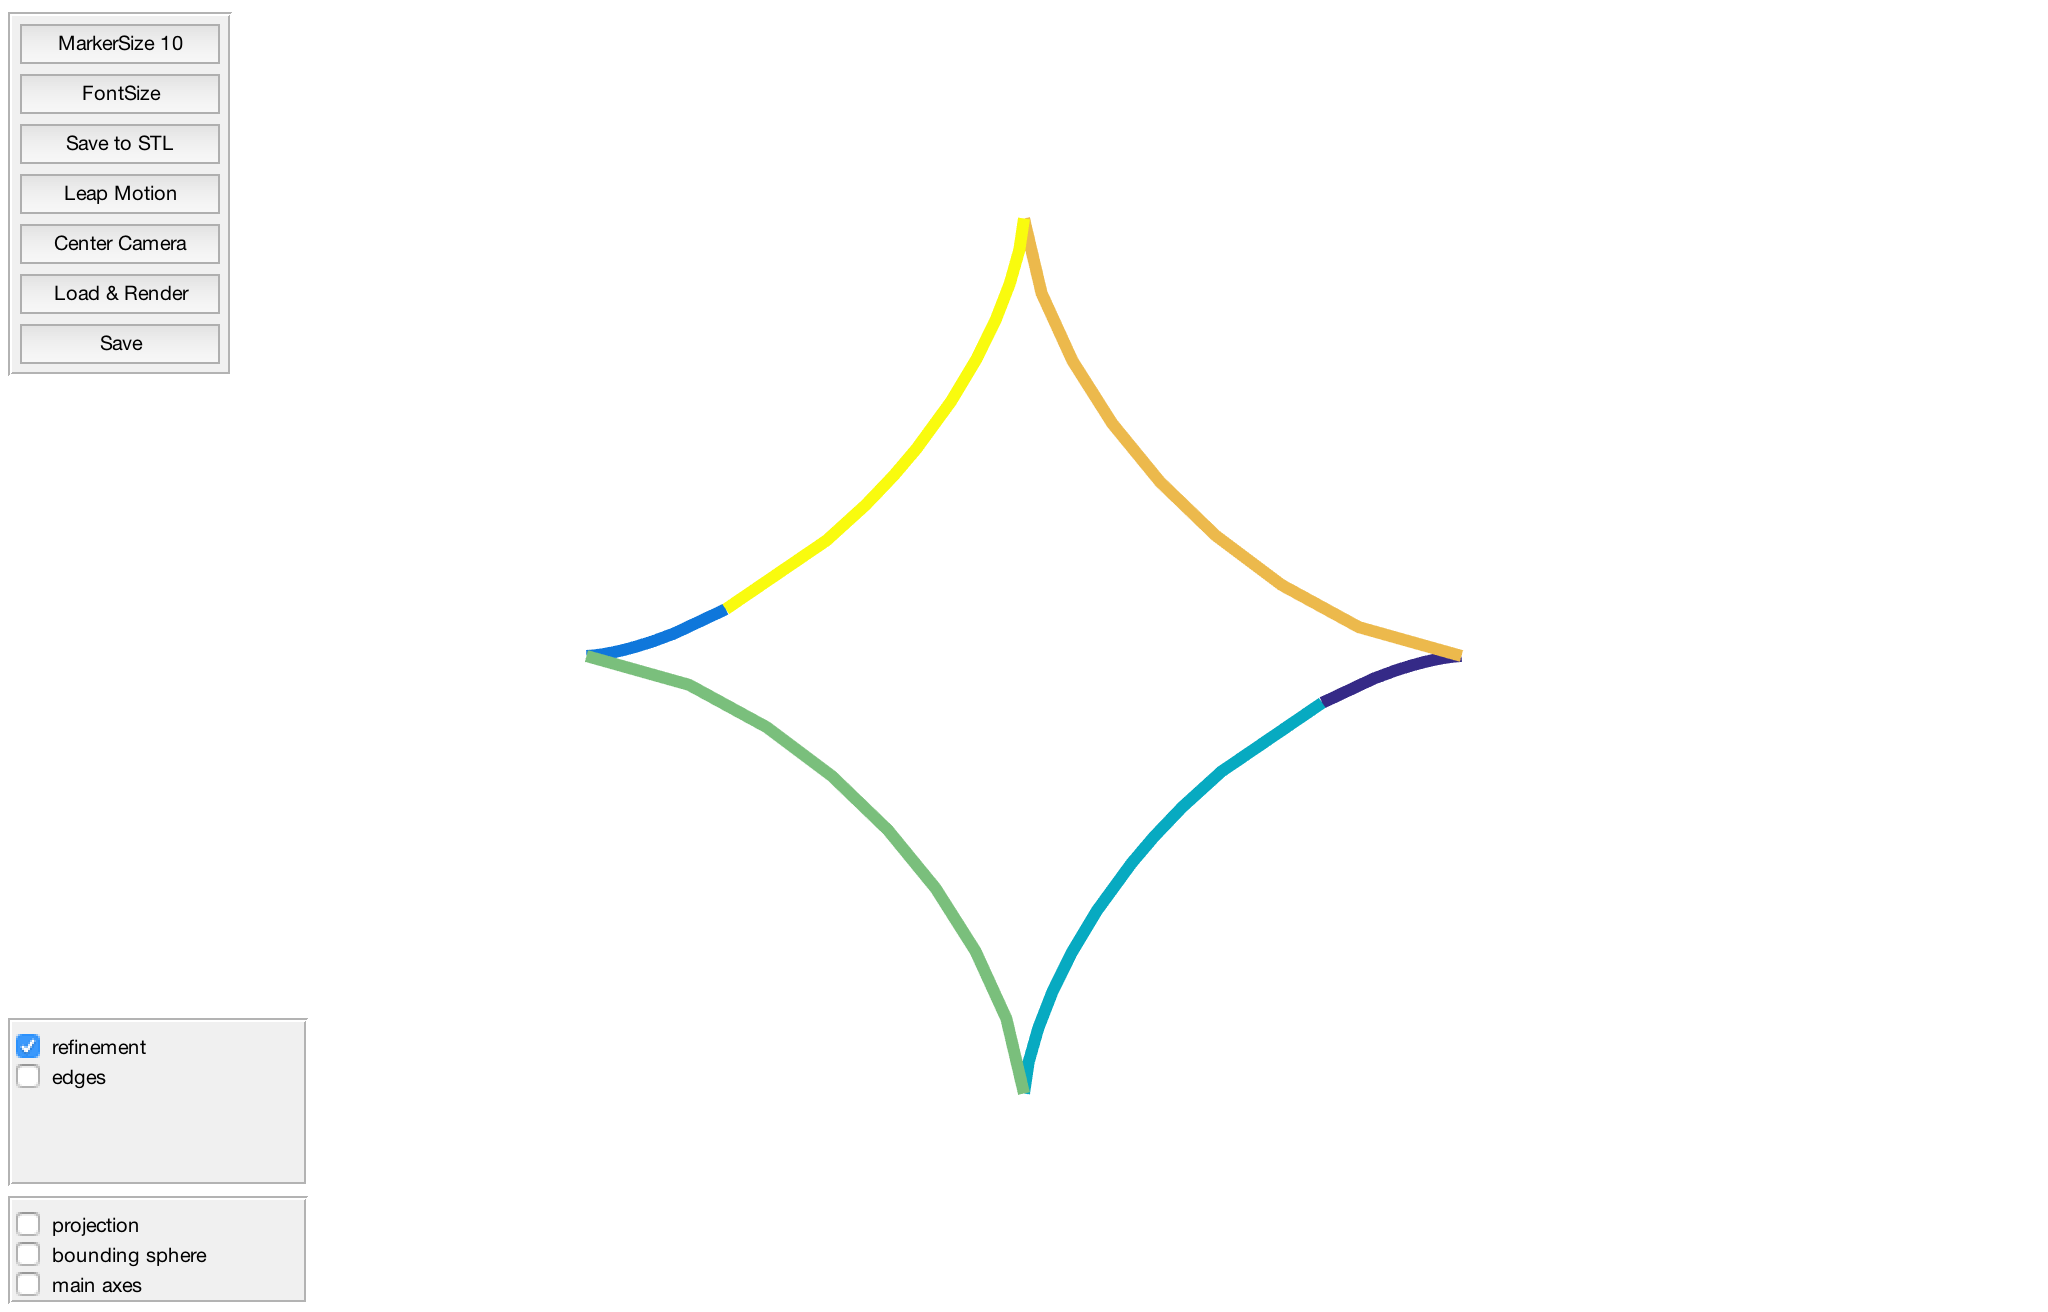
\includegraphics[width=10cm]{example2ref3.png}}
	    \caption{Final astroid plotted}
	\end{figure}

\paragraph{Notes}



\subsection{Surfaces}

\subsubsection{Solitude}

\paragraph{Input file}

	\File{Presents an input file from solitude that instructs Bertini to use all default settings to compute the numerical irreducible decomposition of the sphere in two dimensions}{asdf}{../../test/surface/solitude/input}

\paragraph{Decomposition}
	
	\begin{figure}[H]\centering
	    \frame{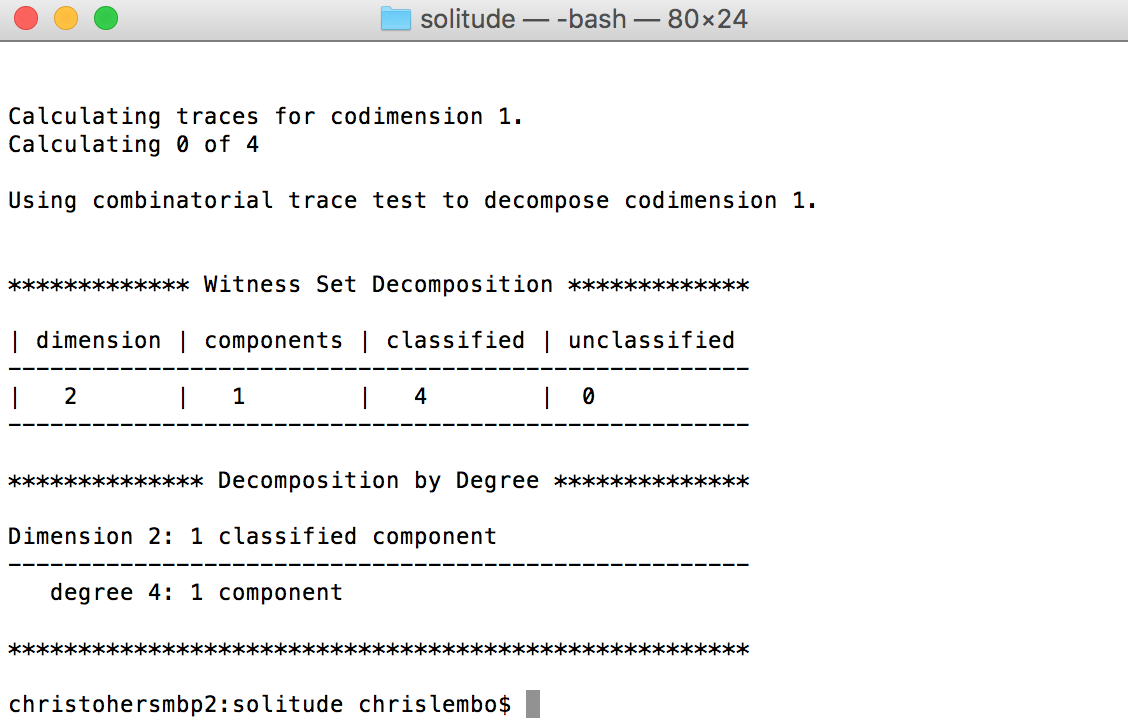
\includegraphics[width=10cm]{example3decomp1}}
	    \caption{Running Bertini using the solitude input file}
	\end{figure}

	\begin{figure}[H]\centering
	    \frame{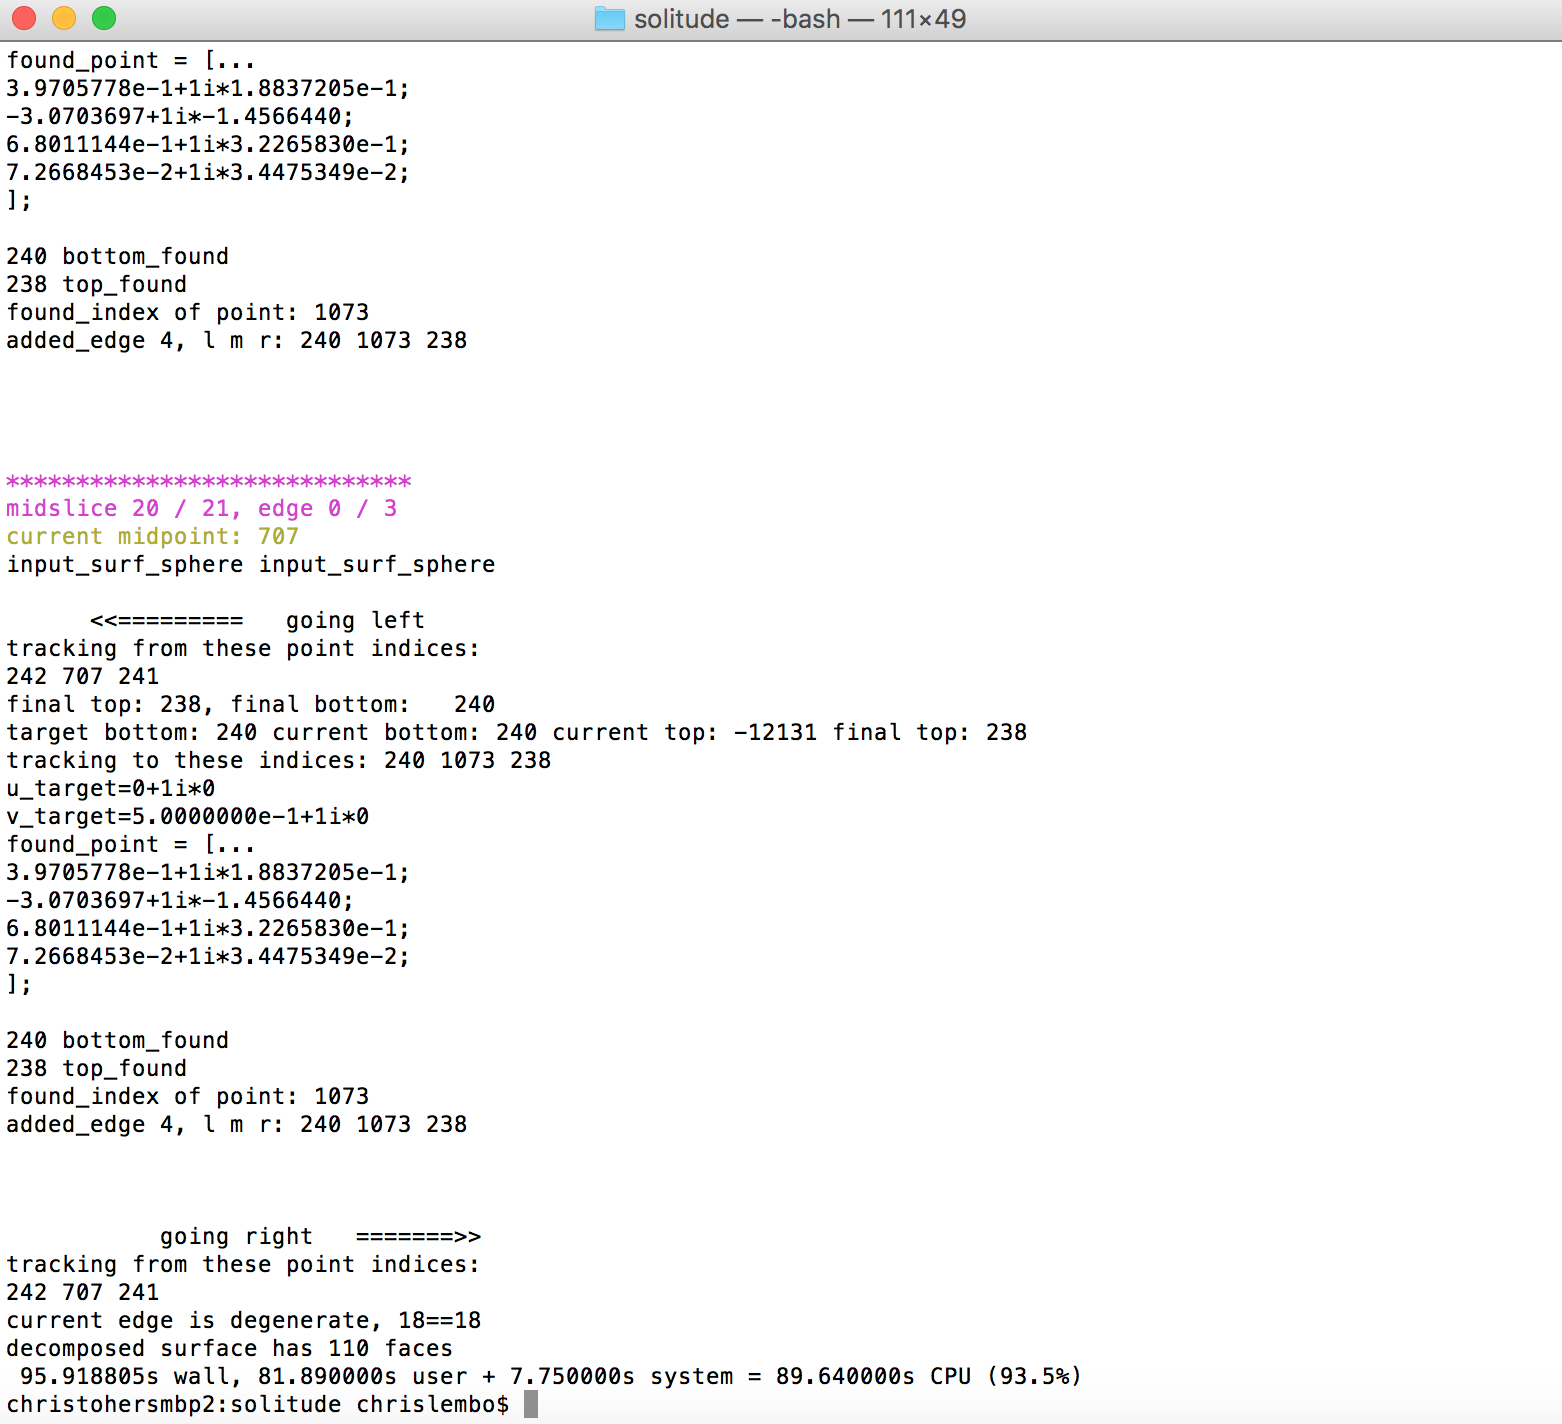
\includegraphics[width=10cm]{example3decomp2}}
	    \caption{Running Bertini\_real using the solitude input file}
	\end{figure}
		
\paragraph{Refinement}

	\begin{figure}[H]\centering
	    \frame{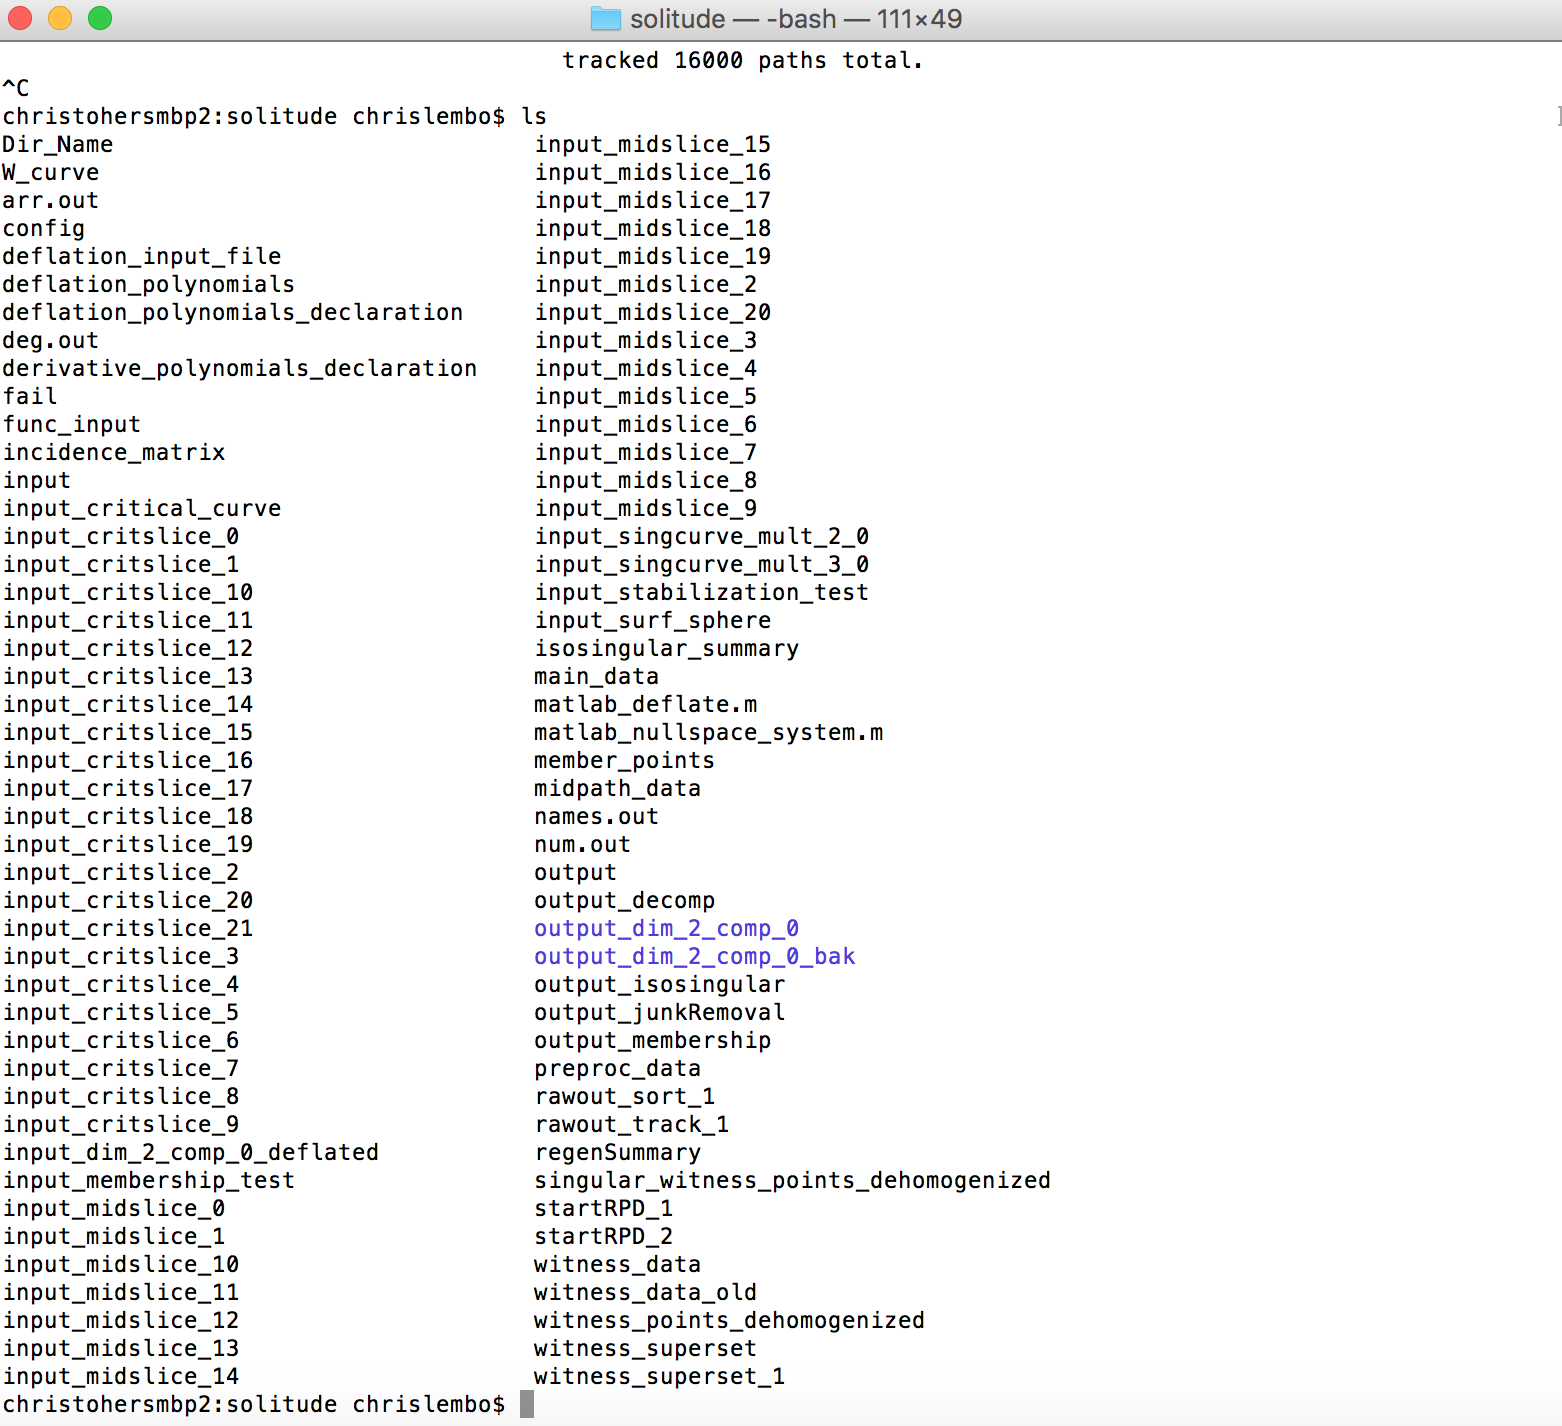
\includegraphics[width=10cm]{example3ref1}}
	    \caption{Refining the solitude input file by invoking sampler using adaptive by distance}
	\end{figure}

	\begin{figure}[H]\centering
	    \frame{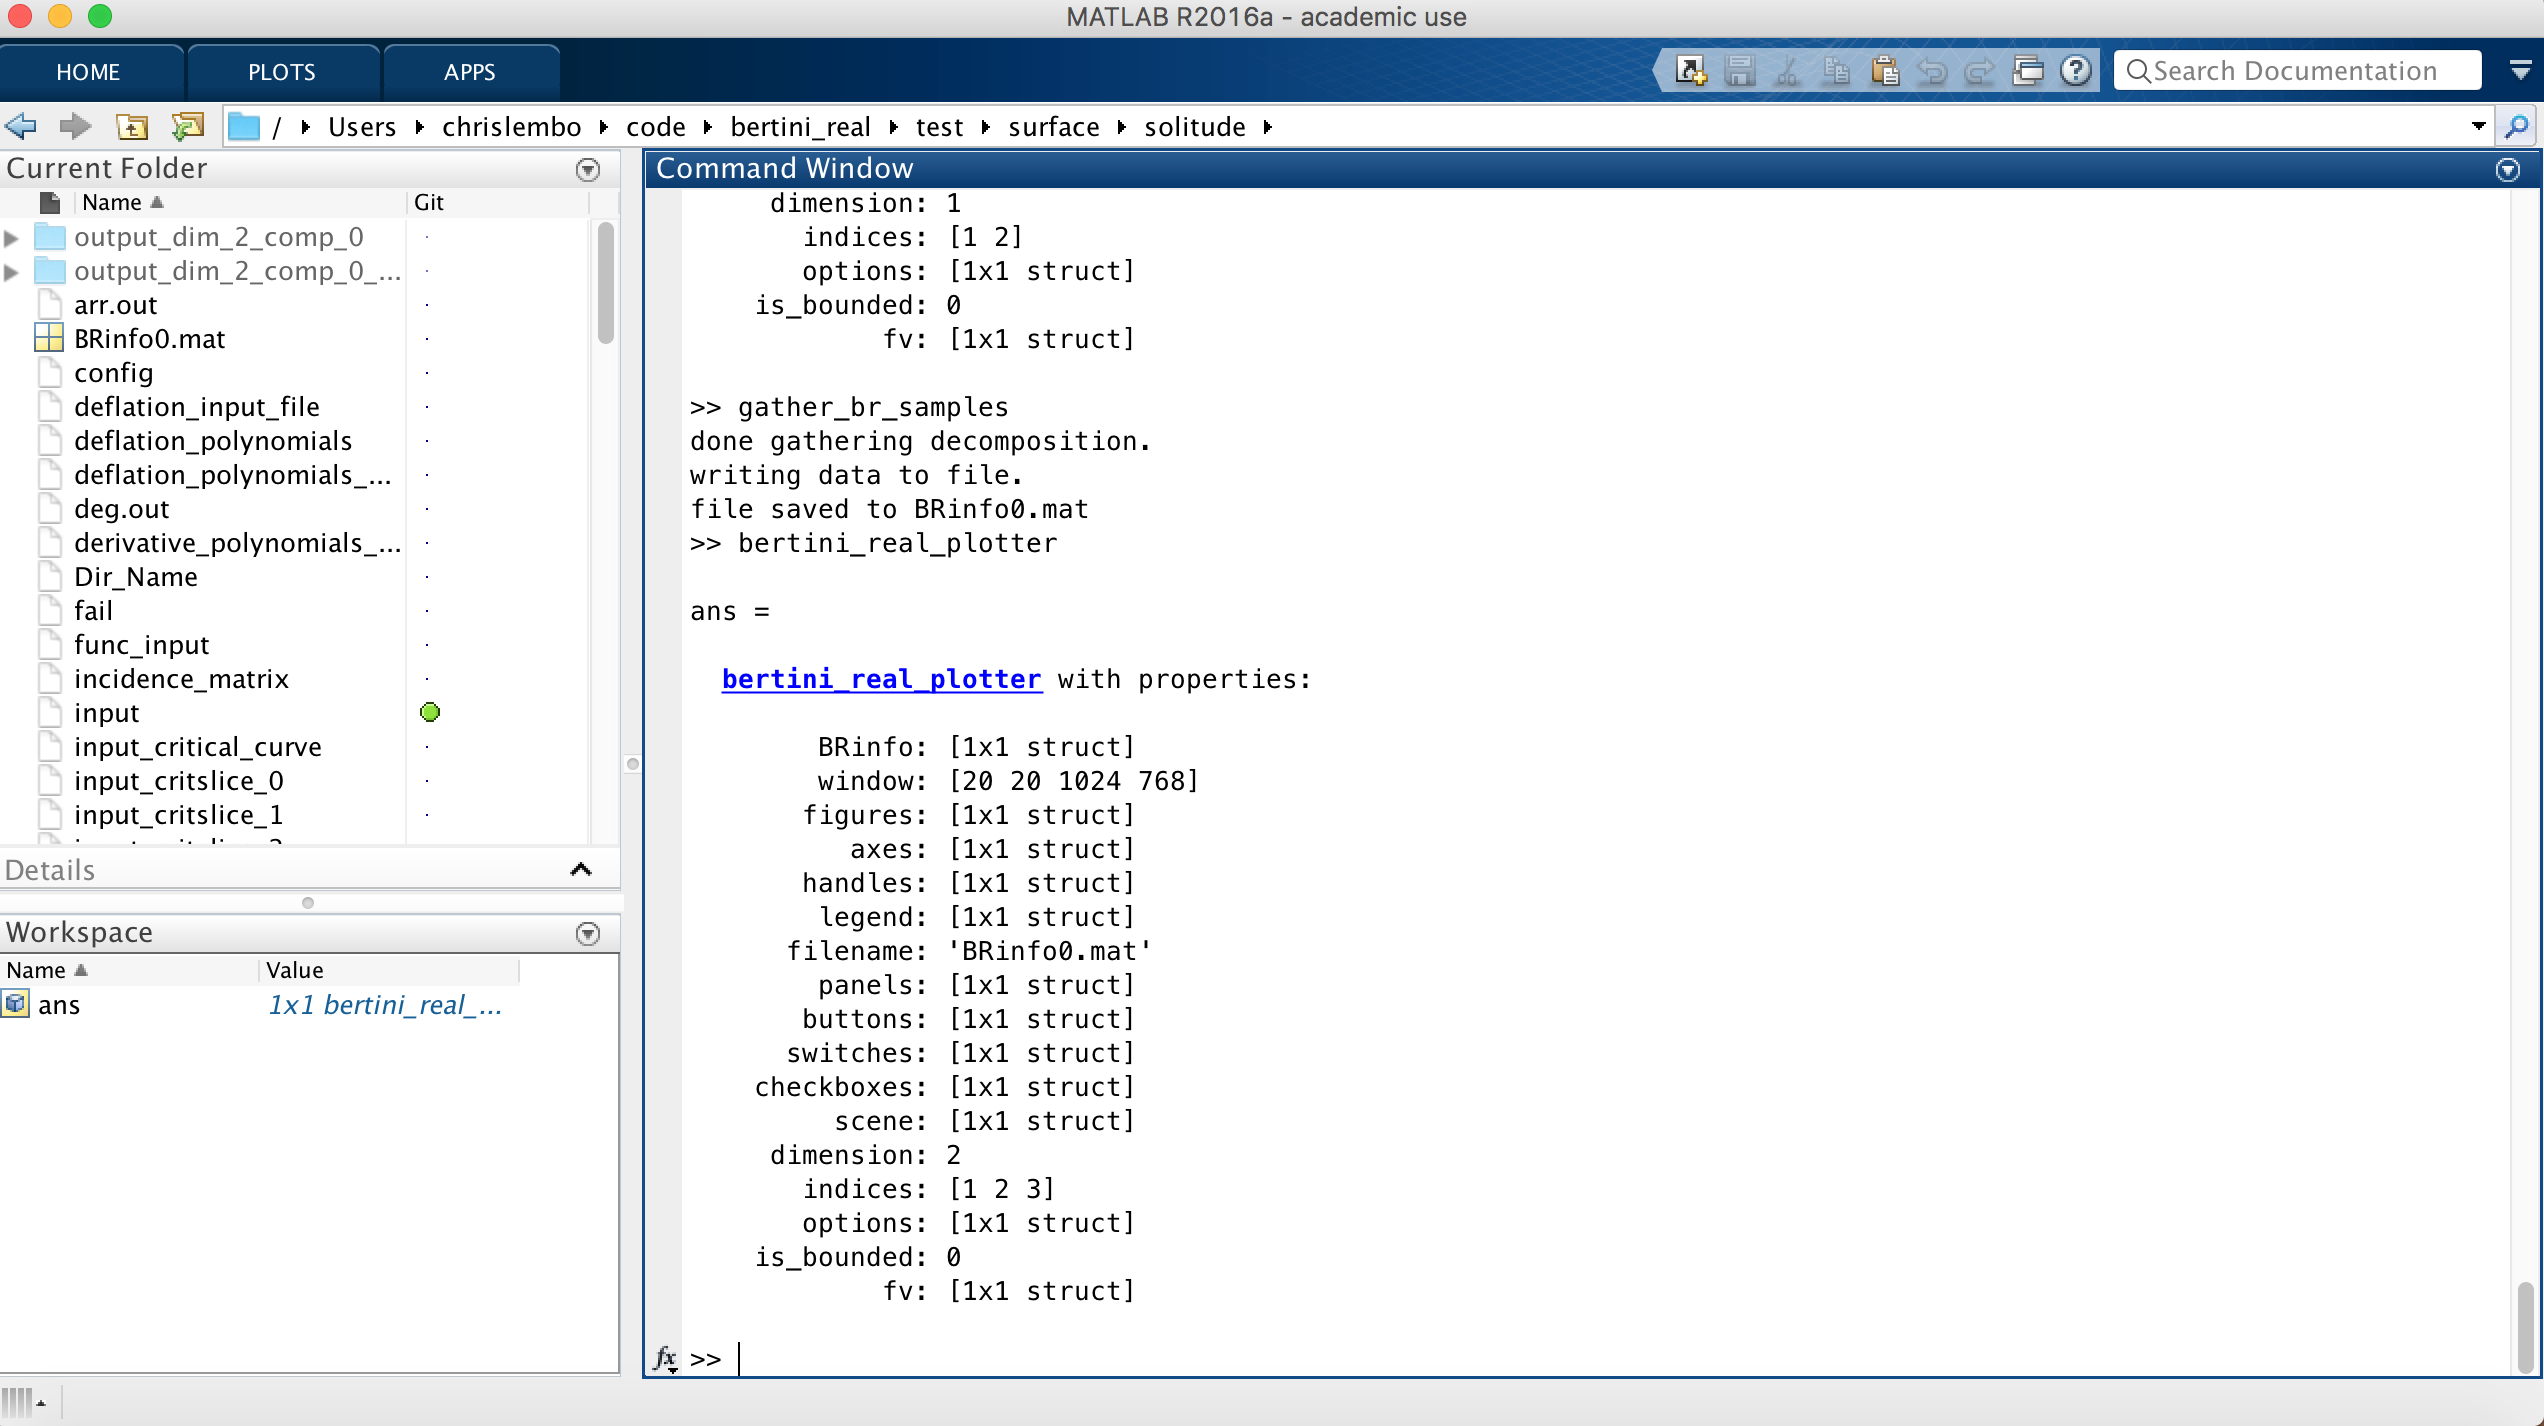
\includegraphics[width=10cm]{example3ref2}}
	    \caption{Gathering and Plotting using MATLAB}
	\end{figure}

	\begin{figure}[H]\centering
	    \frame{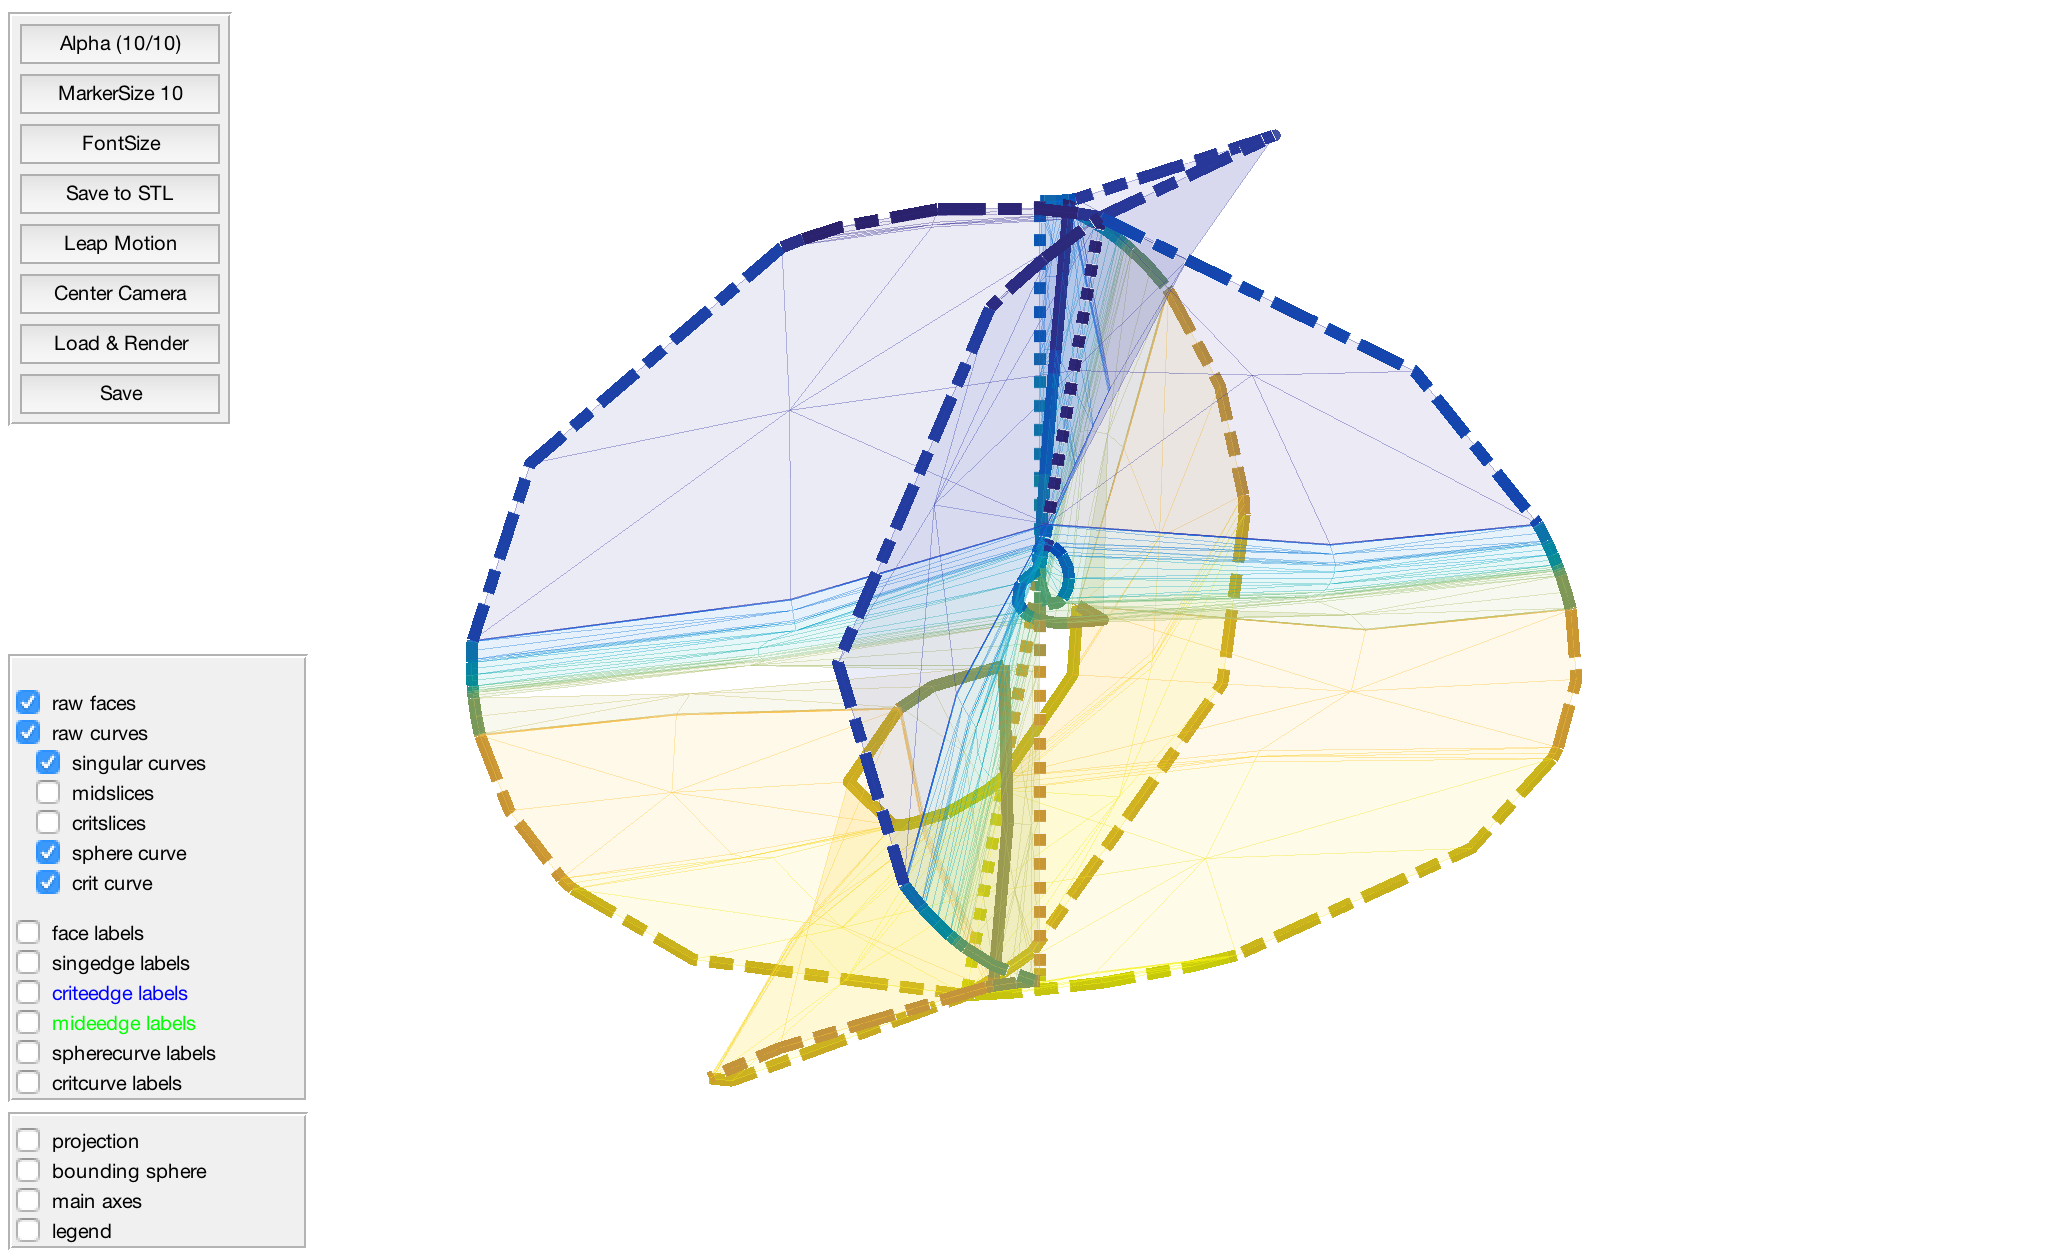
\includegraphics[width=10cm]{example3ref3.png}}
	    \caption{Final solitude plotted}
	\end{figure}

\paragraph{Notes}


---------------------


\subsubsection{Plane}

\paragraph{Input file}

	\File{Presents an input file from plane(note to make this in code writing) that instructs Bertini to use all default settings to compute the numerical irreducible decomposition of the sphere in two dimensions}{asdf}{../../test/surface/plane/input}

\paragraph{Decomposition}
	
	\begin{figure}[H]\centering
	    \frame{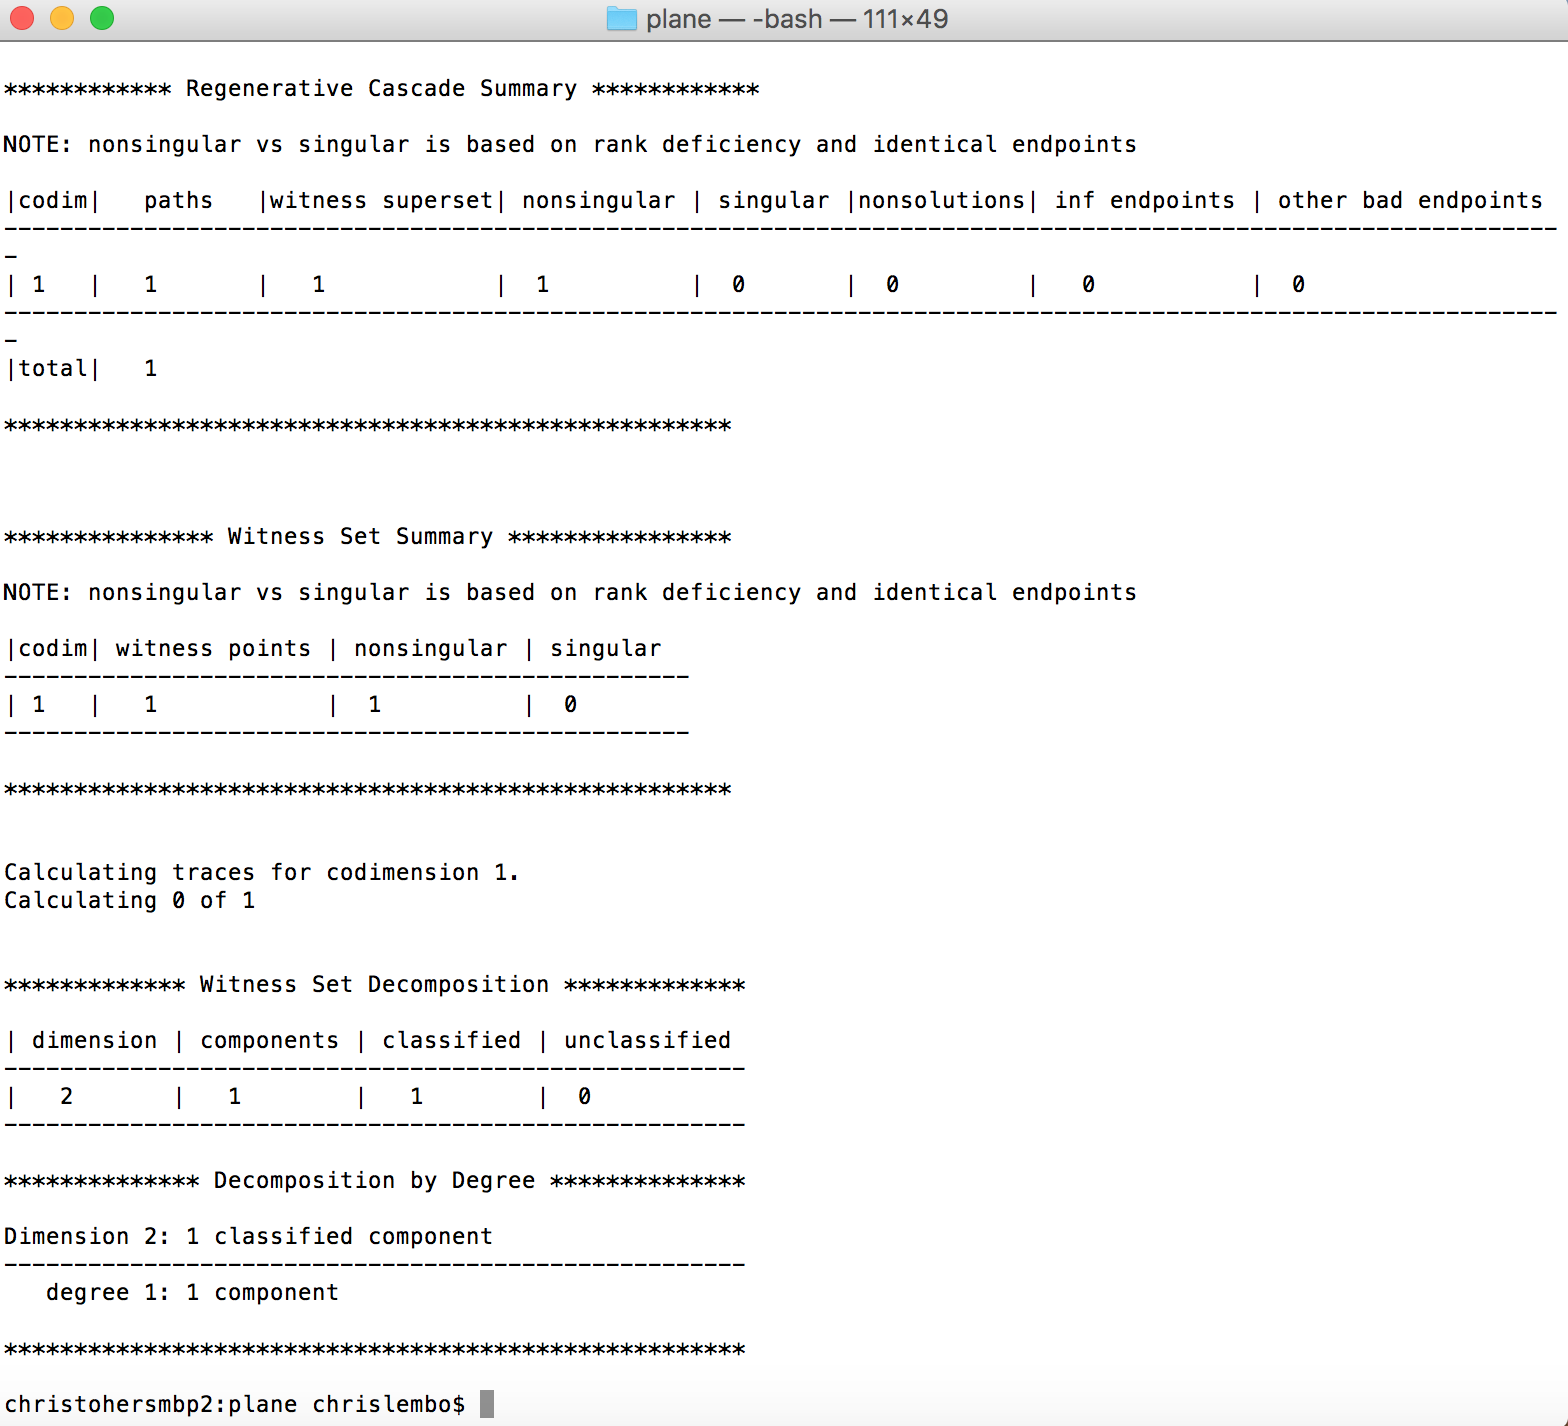
\includegraphics[width=10cm]{example4decomp1}}
	    \caption{Running Bertini using the plane input file}
	\end{figure}

	\begin{figure}[H]\centering
	    \frame{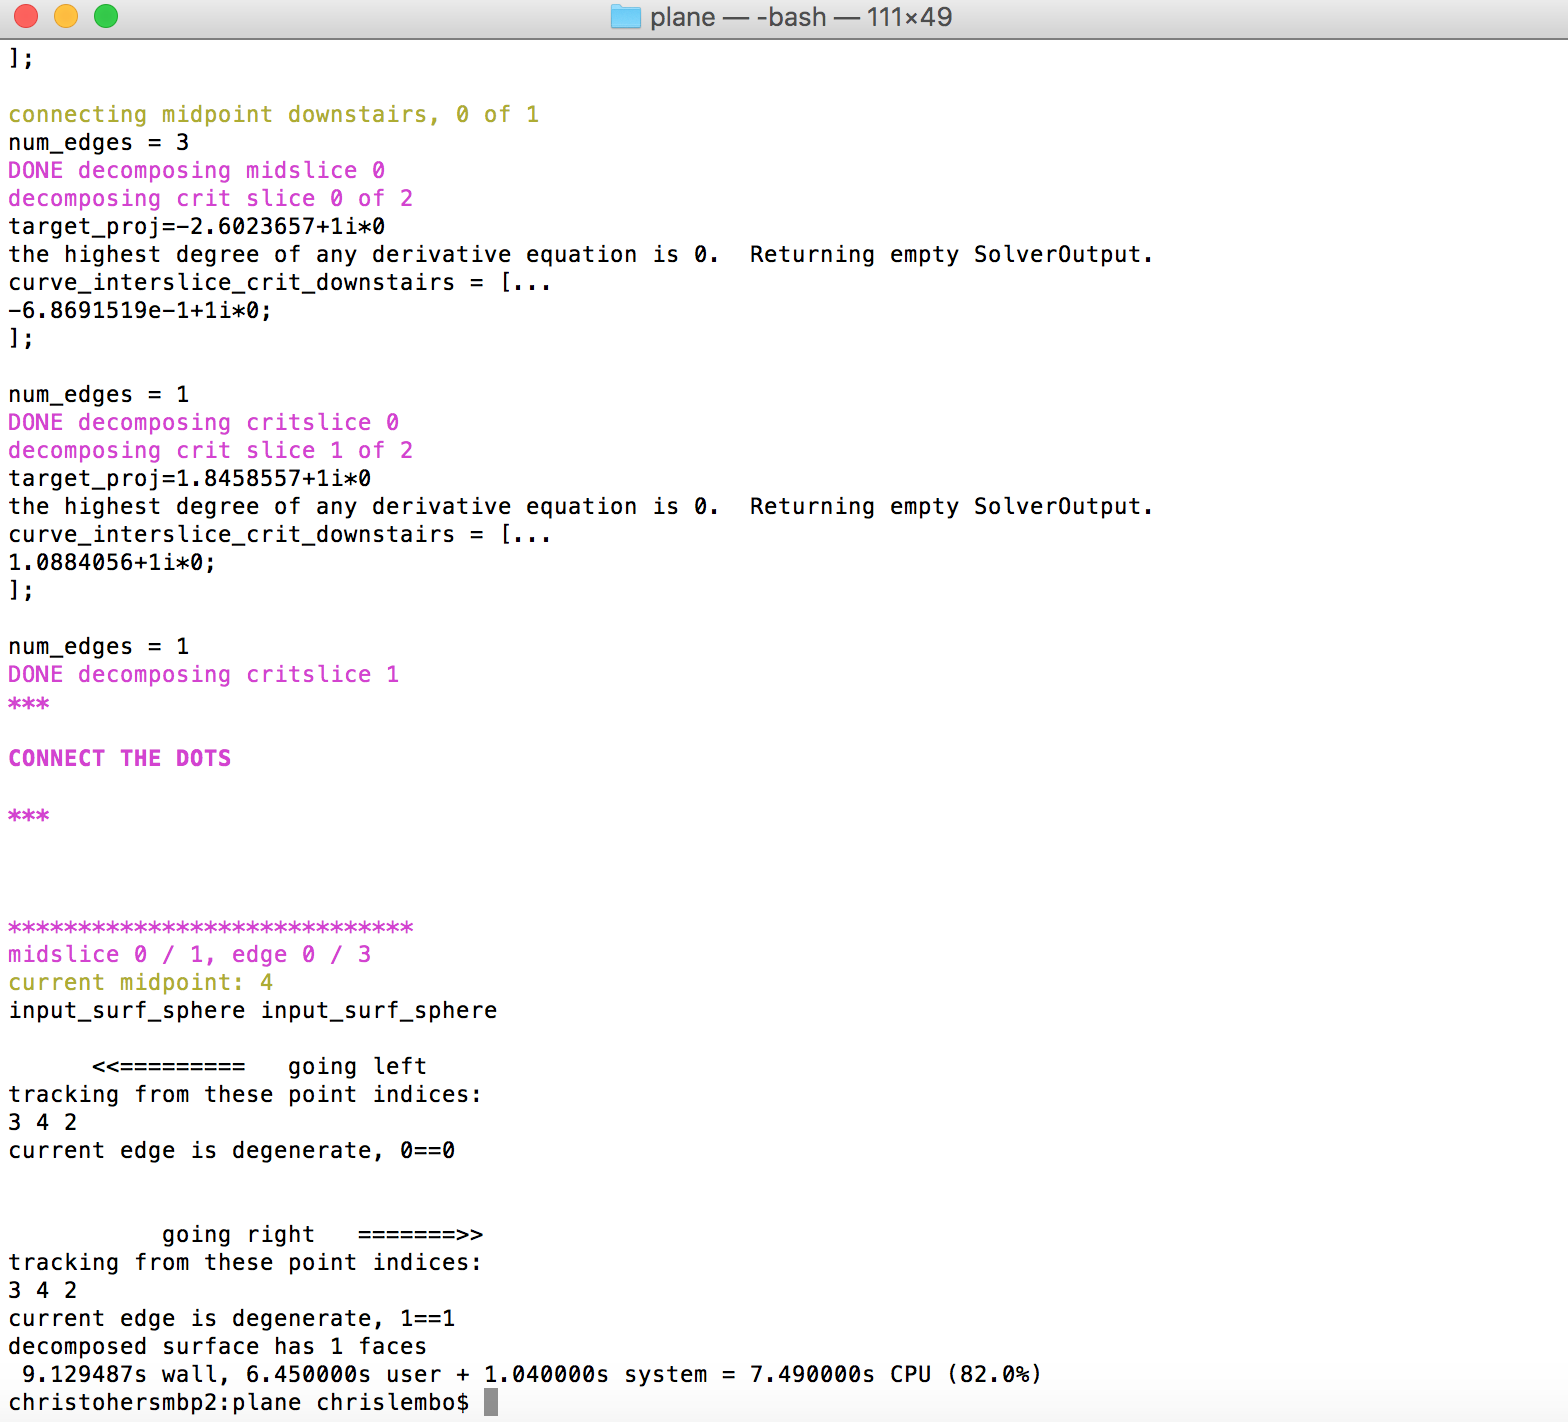
\includegraphics[width=10cm]{example4decomp2}}
	    \caption{Running Bertini\_real using the plane input file}
	\end{figure}
		
\paragraph{Refinement}

	\begin{figure}[H]\centering
	    \frame{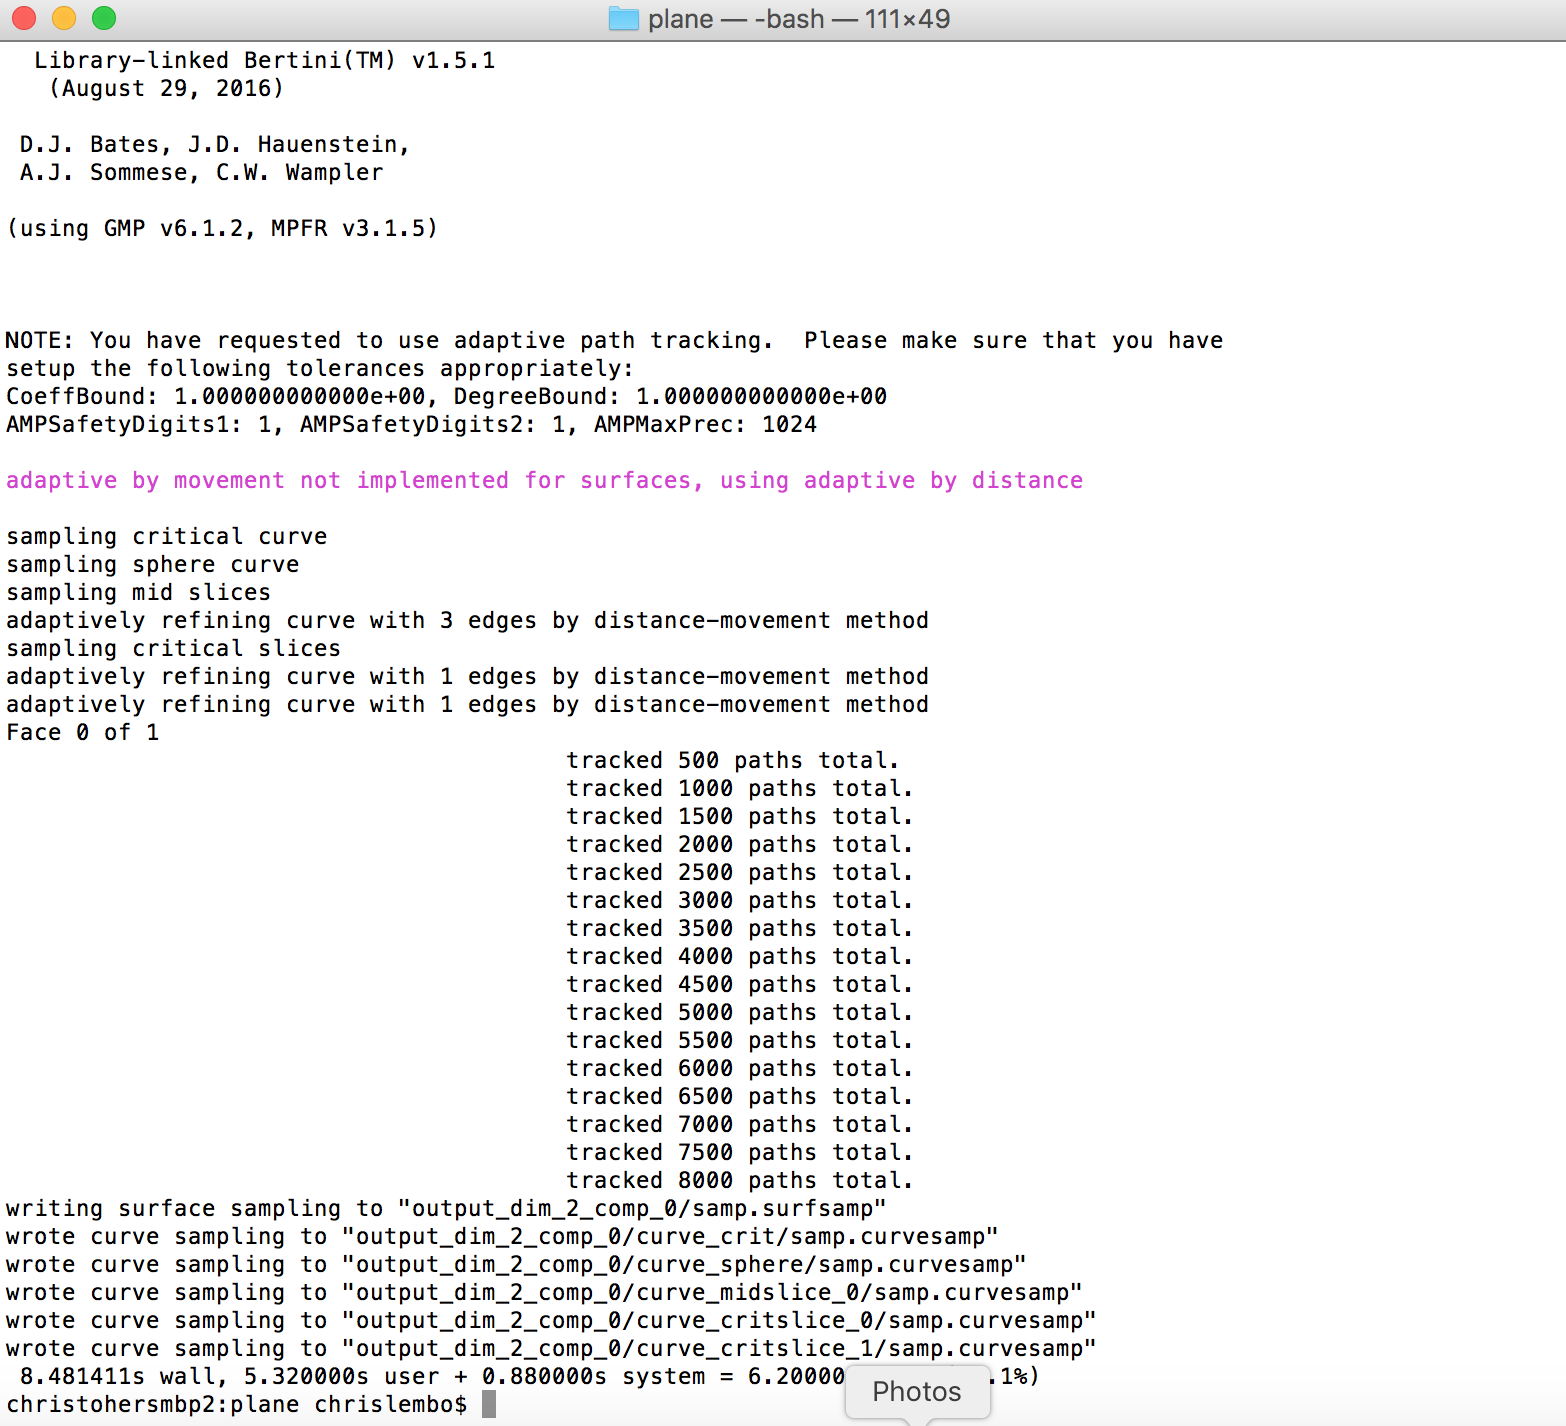
\includegraphics[width=10cm]{example4ref1}}
	    \caption{Refining the plane input file by invoking sampler}
	\end{figure}

	\begin{figure}[H]\centering
	    \frame{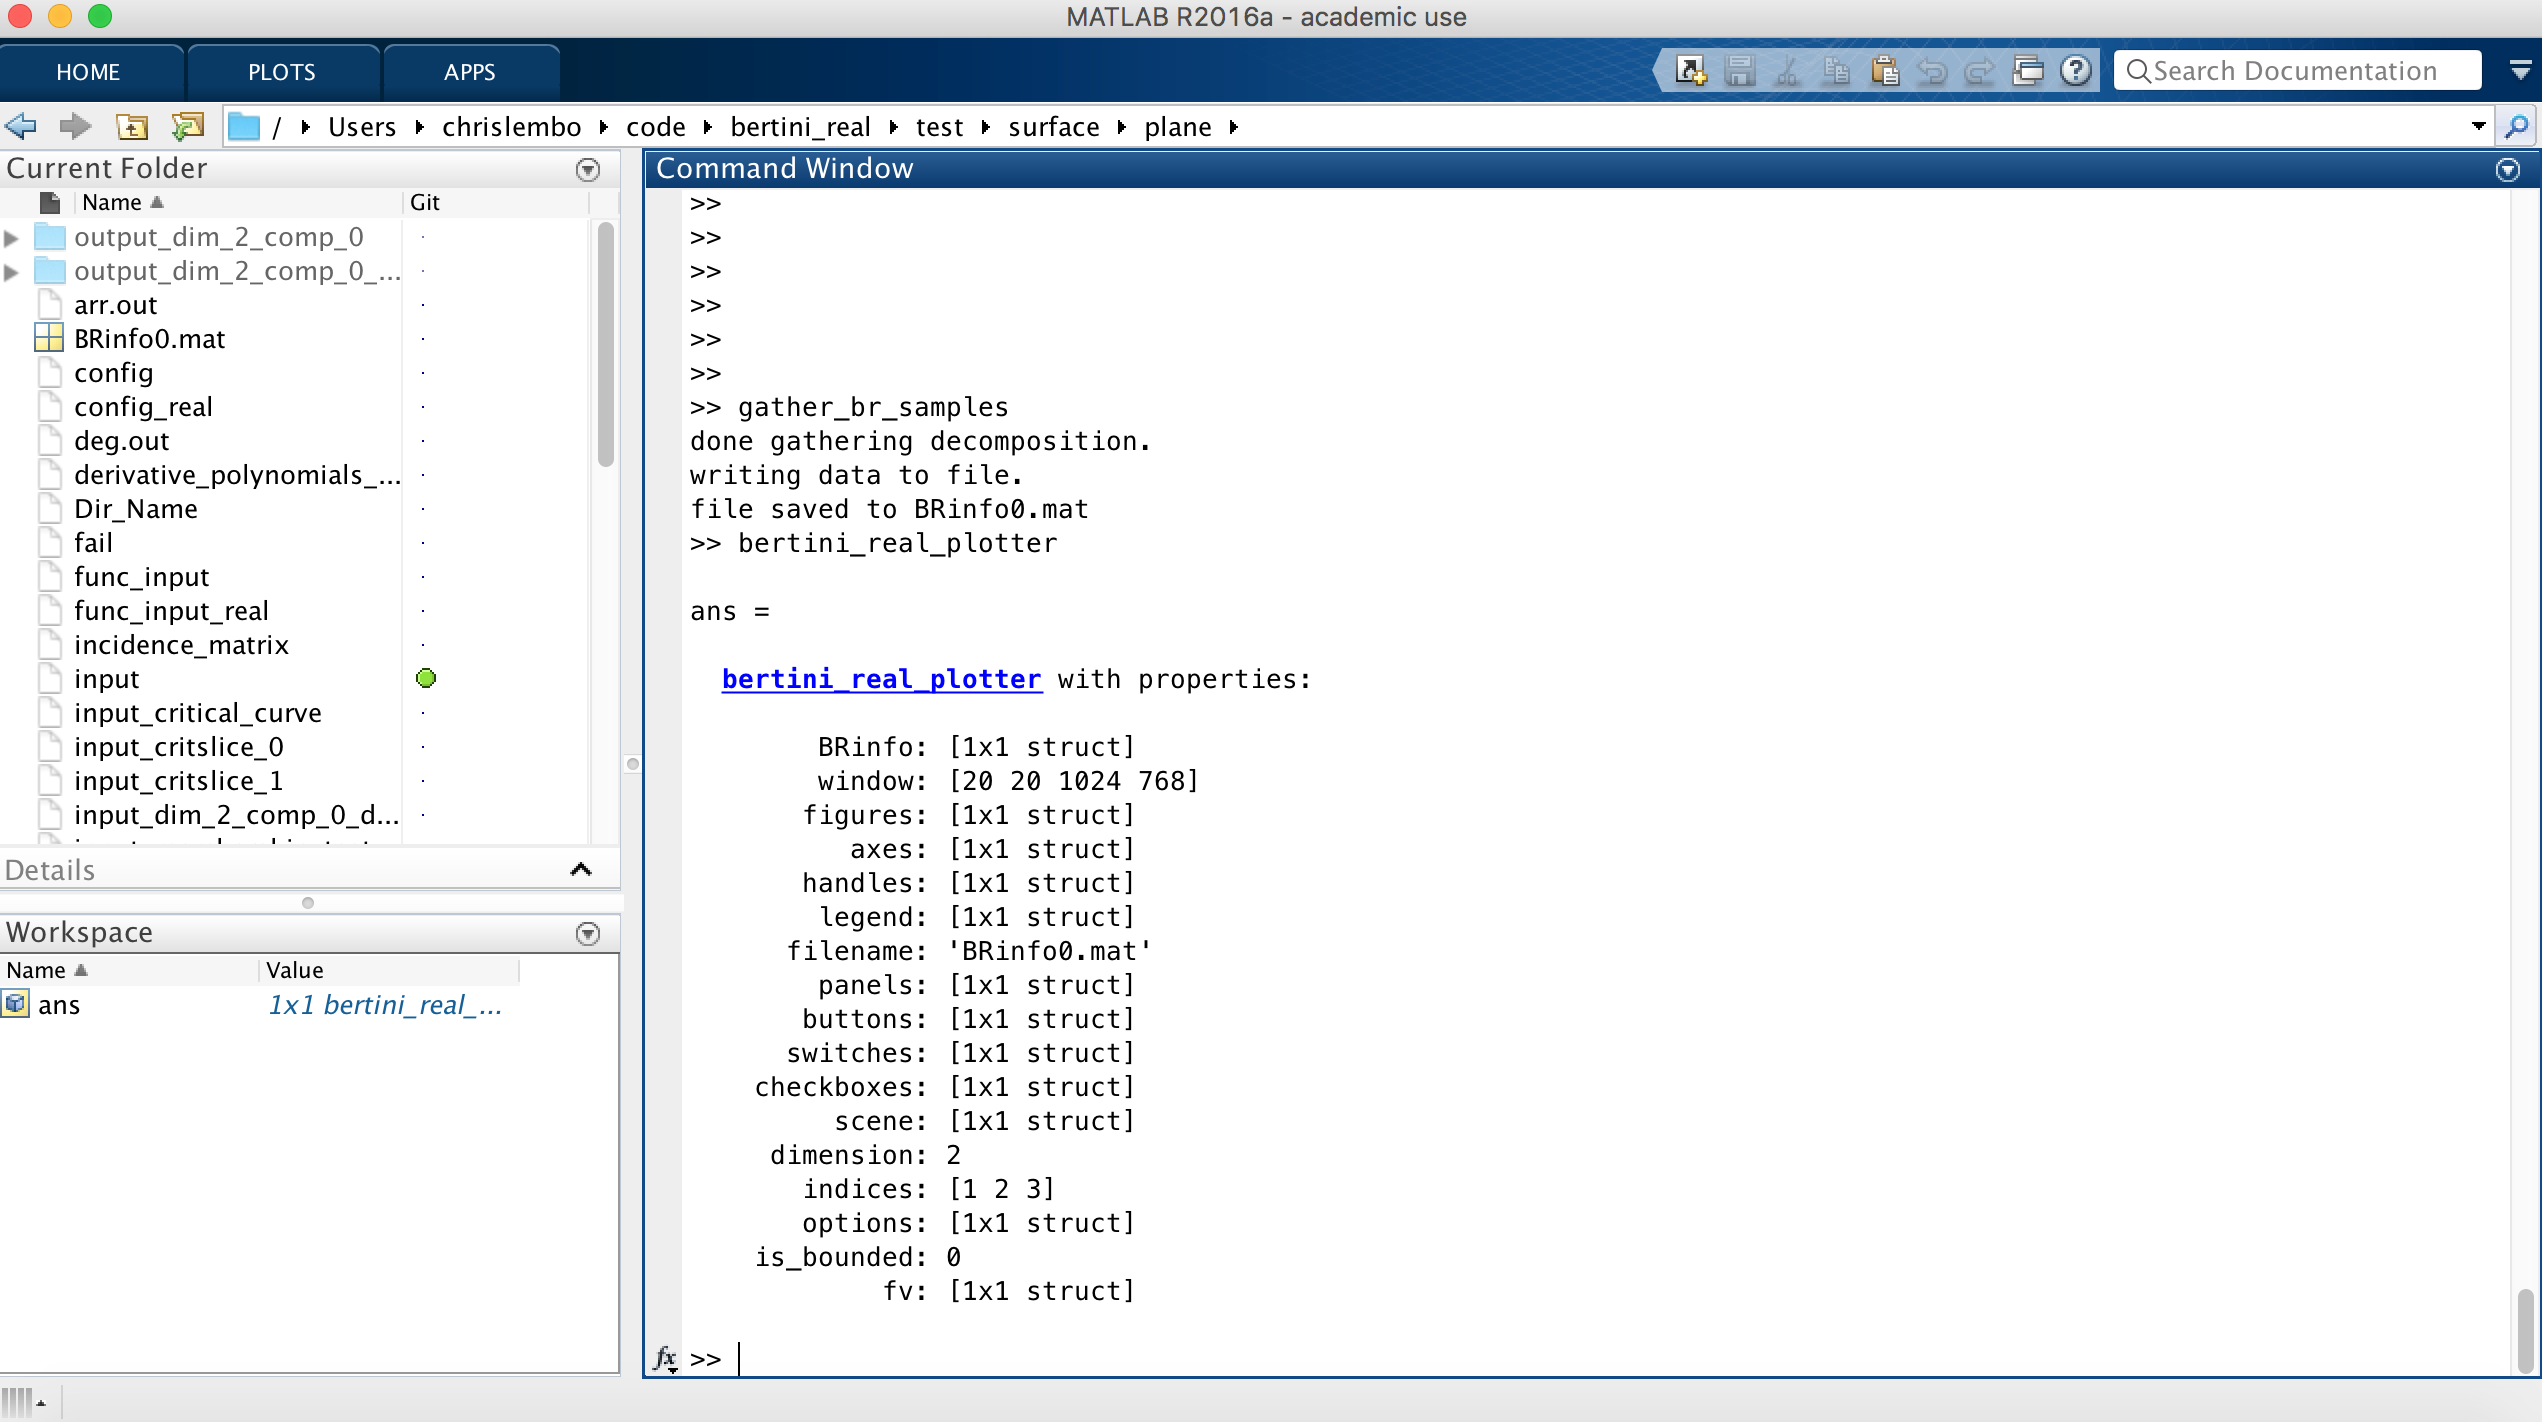
\includegraphics[width=10cm]{example4ref2}}
	    \caption{Gathering and Plotting using MATLAB}
	\end{figure}

	\begin{figure}[H]\centering
	    \frame{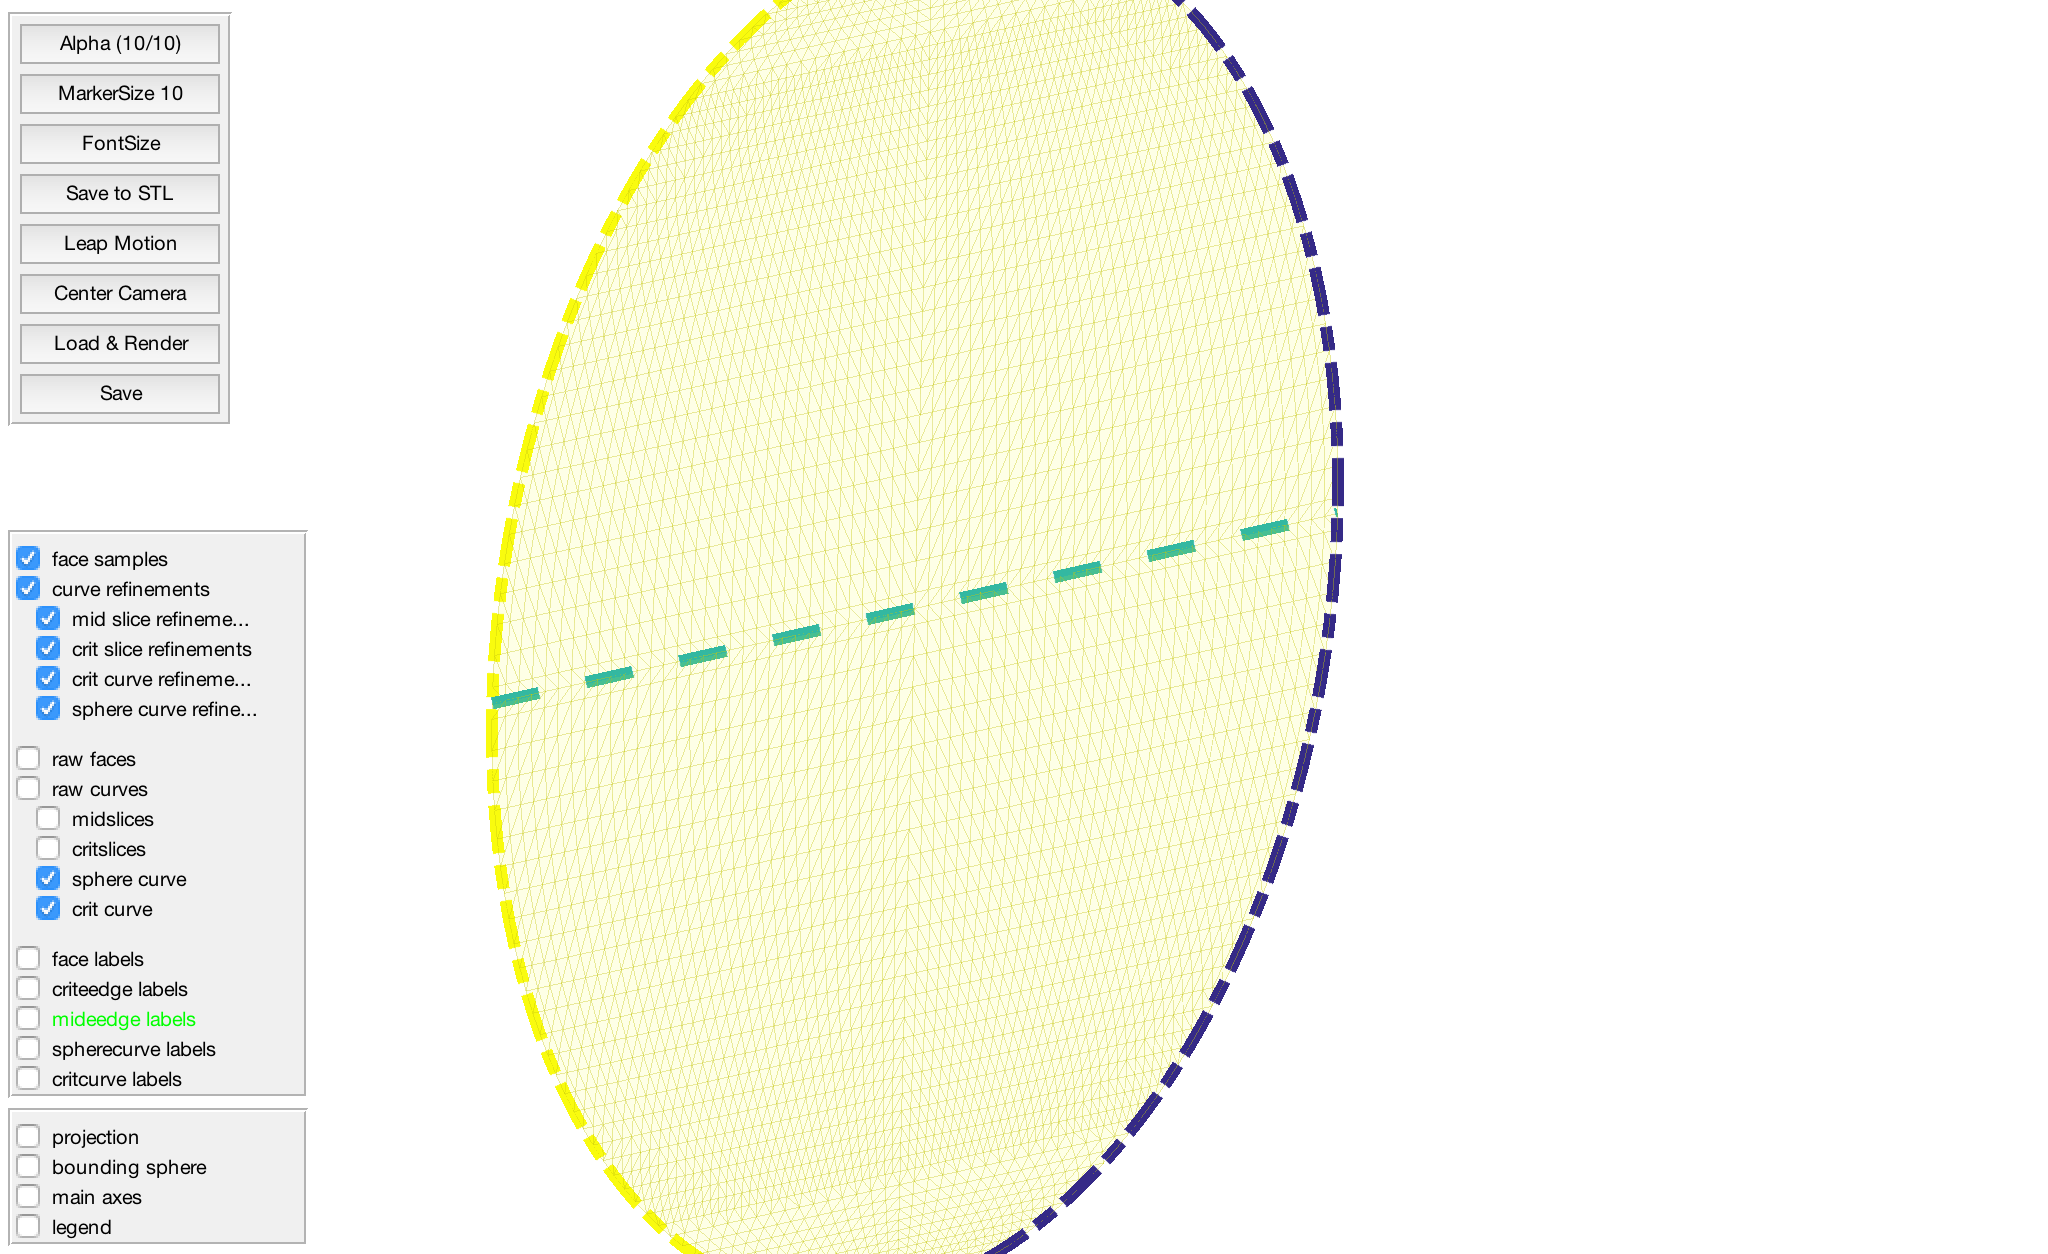
\includegraphics[width=10cm]{example4ref3.png}}
	    \caption{Final plane plotted}
	\end{figure}

\paragraph{Notes}



